\documentclass[10pt,xcolor=table]{beamer}

\usetheme[subsectionpage=none]{metropolis}
%\useoutertheme{infolines}
%HEADEEER
\makeatletter

%HEADER
%\setbeamertemplate{headline}{%
%  \begin{beamercolorbox}[colsep=1.5pt]{upper separation line head}
%  \end{beamercolorbox}
%  \begin{beamercolorbox}{section in head/foot}
%    \vskip2pt\insertnavigation{\paperwidth}\vskip0pt
%  \end{beamercolorbox}%
%  \begin{beamercolorbox}[colsep=1.5pt]{lower separation line head}
%  \end{beamercolorbox}
%}
%\def\beamer@writeslidentry{\clearpage\beamer@notesactions}

%SECTION PAGES (HEAD then COMPLETE title)
\defbeamertemplate*{section page}{mytheme}{
  \centering
  \begin{minipage}{22em}
    \raggedright
    \usebeamercolor[fg]{section title}
    \usebeamerfont{section title}
    \insertsectionhead\\[-1ex]
    \vspace{1cm}
    \usebeamerfont{subsection title}
    \insertsection\textit{}\\[-1ex]
    \usebeamertemplate*{progress bar in section page}
    \par
    \ifx\insertsubsectionhead\@empty\else%
      \usebeamercolor[fg]{subsection title}%
      \usebeamerfont{subsection title}%
      \insertsubsectionhead
    \fi
    \vskip0.5cm
   
  \end{minipage}
  \par
  \vspace{\baselineskip}
}
%SUBSECTIONN PAGE (only subsection title)

\makeatother


\usepackage{appendixnumberbeamer}
\usepackage{booktabs}
\usepackage{multirow}
\usepackage{forest} 
\usepackage{adjustbox}
\usepackage{mathtools}
\usepackage{tikz}
\newcommand*\circled[1]{\tikz[baseline=(char.base)]{
            \node[shape=circle,draw,inner sep=1pt] (char) {#1};}}

%\usepackage[scale=2]{ccicons}

\usepackage[backend=bibtex,style=alphabetic,sorting=ynt]{biblatex}
\addbibresource{Thesis_f.bib}

\usepackage{pgfplots}
\usepgfplotslibrary{dateplot}

\usepackage{xspace}
\newcommand{\themename}{\textbf{\textsc{metropolis}}\xspace}

% \usepackage[T1]{fontenc} 
% \usepackage[latin1]{inputenc}
% \usepackage[frenchb]{babel}
\usepackage{FiraSans}
 

\usepackage[ruled]{algorithm2e}

\SetKwRepeat{Do}{do}{while}%
\SetKwInput{KwInput}{Input}
\SetKwInput{KwOutput}{Output}

\hbadness=10000


\usepackage{url}

\usepackage{graphicx}
% % % % % % % % % % % % % % % % % % %DEFINITIONS MINE
\newcommand\mlex{M^{\scriptscriptstyle L}}
\newcommand\msyn{M^{\scriptscriptstyle S}}
\newcommand\mstd{M^{\scriptscriptstyle T}}
\newcommand\slex{S^{\scriptscriptstyle L}}
\newcommand\ssyn{S^{\scriptscriptstyle S}}
\newcommand\sstd{S^{\scriptscriptstyle T}}

\newcommand{\stackwords}[2]{\begin{tabular}[t]{@{}l@{}}#1\\#2\end{tabular}}

\title{\large Hypergraphs and Information Fusion for Term Representation Enrichment. Applications to Named Entity Recognition and Word Sense Disambiguation}
\subtitle{\normalsize  Ph.D. Thesis Defense}

% \\ 
%February 7th 2018 \\ 
%Supervisor: Sabine Loudcher \\
%Co-supervisor: Julien Ah-Pine \\ 
%Laboratoire ERIC \\ Universit\'{e} Lumi\`{e}re Lyon 2}
\date[February 7th, 2018]{February 7th, 2018}
\author[Pavel SORIANO-MORALES]{\normalsize Pavel Soriano-Morales\\{Supervised by Sabine Loudcher and Julien Ah-Pine}}

\institute{
	 \vspace{15mm} % 
	\begin{center}
      
\includegraphics[height=0.9cm]{Logo/Logo_Lyon_1}% Logo Lyon 1
      
\includegraphics[height=0.9cm]{Logo/Logo-Lyon2}% Logo Lyon 2 
      
\includegraphics[height=0.9cm]{Logo/Logo-udl}% Logo Univ Lyon
      
\includegraphics[height=0.9cm]{Logo/Logo_ISH}% Logo ISH
      
      \end{center}
      }
 \titlegraphic{\vspace{6mm}\hfill
\includegraphics[height=1.3cm]{Logo/4_Logo_ERIC_avec_baseline}} % Logo ERIC
  
\begin{document}

\metroset{sectionpage=none}
\maketitle


\section{Introduction}
\metroset{sectionpage=progressbar}
\begin{frame}{Why it is useful to us to understand text?}
%	\large  \textbf{Why it is useful to us to automatically understand written language?} \hfill
	\vspace{1cm}
	\begin{columns}
	\column{0.5\textwidth}
	\begin{minipage}[c][0.5\textheight][c]{\linewidth}
	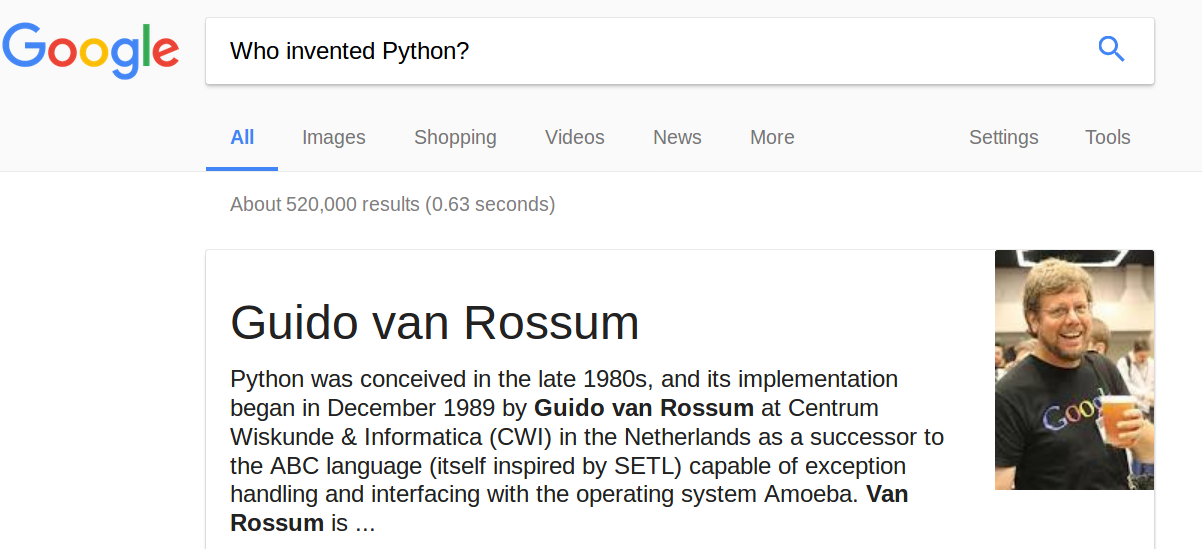
\includegraphics[width=1\linewidth]{image2/Chapitre1/guido_google.png}
	\end{minipage}
	\column{0.5\textwidth}
	\begin{minipage}[c][0.5\textheight][c]{\linewidth}
	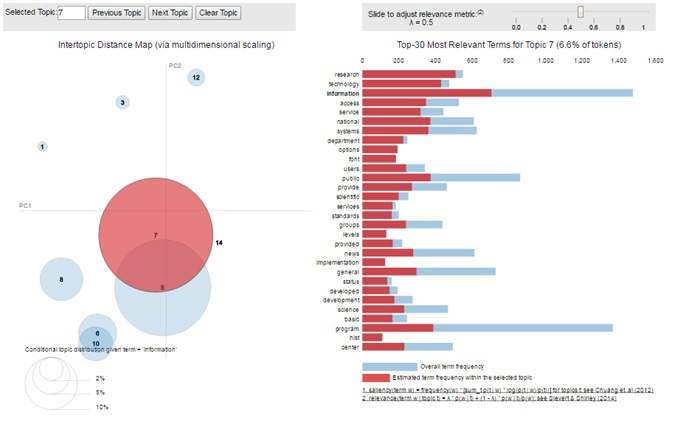
\includegraphics[width=1\linewidth]{image2/Chapitre1/lda_2d.jpg}
	\end{minipage}
	\end{columns}
	\vspace{\textheight}
\end{frame}

\begin{frame}{How do we extract meaning from text?}
%\vspace{1cm}

\begin{itemize}
\item[] {{We use \textbf{Natural Language Processing} (NLP), a field of computer science interested on making computers extract useful information from text}}
\end{itemize}
\begin{figure}
\centering
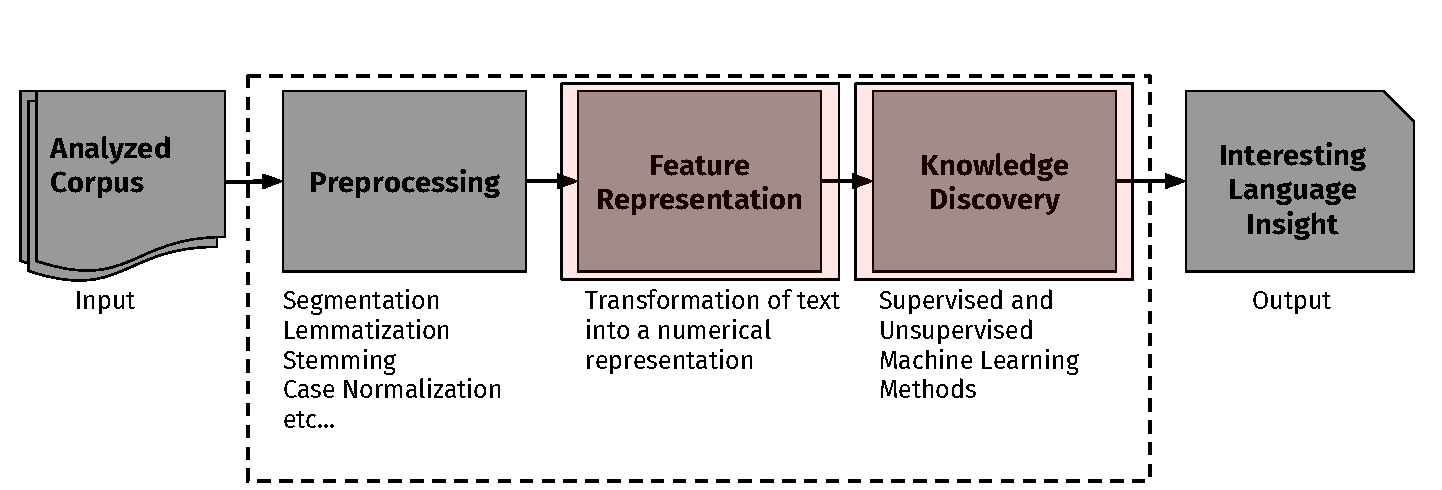
\includegraphics[width=1\linewidth]{image2/Chapitre1/nlp_flow2}
\end{figure}
\vspace{\textheight}
\end{frame}

	
\begin{frame}
\frametitle{Feature Representation and Knowledge Discovery}
%\vspace{1cm}


\begin{columns}
\column{0.5\textwidth}
\begin{itemize}
\item[] How do we represent text for the machine to understand? 
\end{itemize}
\begin{minipage}[c][0.5\textheight][c]{\linewidth}
\centering
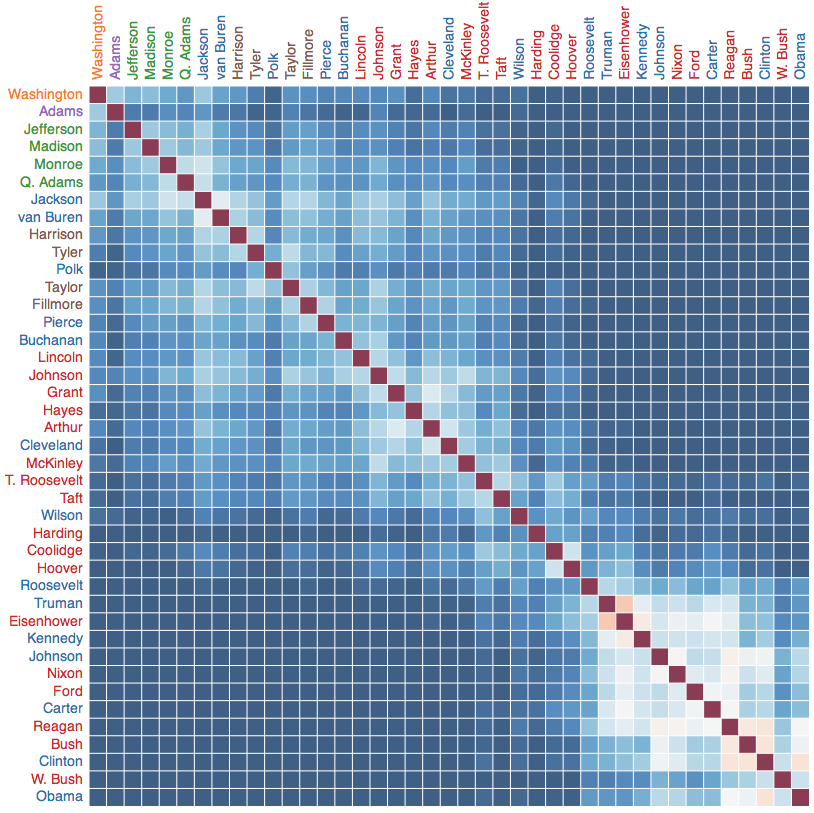
\includegraphics[width=.7\linewidth]{image2/Chapitre1/matrix.png}
\end{minipage}
\column{0.5\textwidth}
\begin{itemize}
\item[] What techniques do we use to discover meaning from text?
\end{itemize}
\begin{minipage}[c][0.5\textheight][c]{\linewidth}
\centering
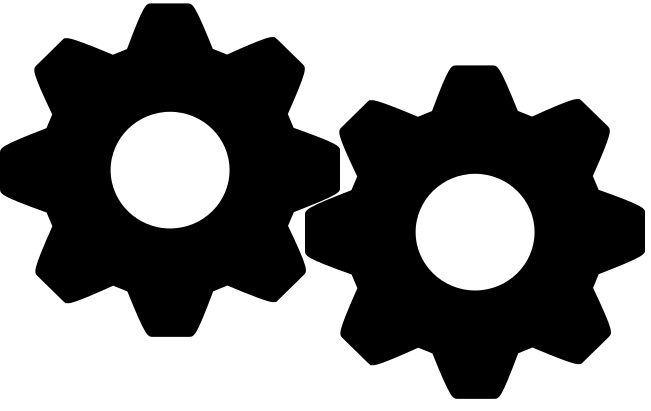
\includegraphics[width=.8\linewidth]{image2/Chapitre1/kdisc.png}
\end{minipage}
\end{columns}

\vspace{\textheight}

\end{frame}
%\subsection{Challenges and Contributions}

\begin{frame}{Representing Text}
%So for example, in this text, I can get features that describe its properties. They may be lexical (needing only the information of the words surrounding each word), syntactical (exaplin syntactic vs dependency tree)

\begin{itemize}[<+- | alert@+>]
	\item \textbf{Three common ways to represent text}
	\begin{itemize}
		\item Lexical
		\item Syntactic
		\begin{itemize}
				\item Constituency Tree
				\item Dependency Tree
		\end{itemize}
	\end{itemize}
	\item \textbf{Working Example}
	\begin{itemize}
		\item[] \textit{The report contains copies of the minutes of these meetings}
	\end{itemize}
\end{itemize}

\begin{overprint}
  				
  \onslide<8>
%	  \textbf{Lexical Information}

	  \centering	  
      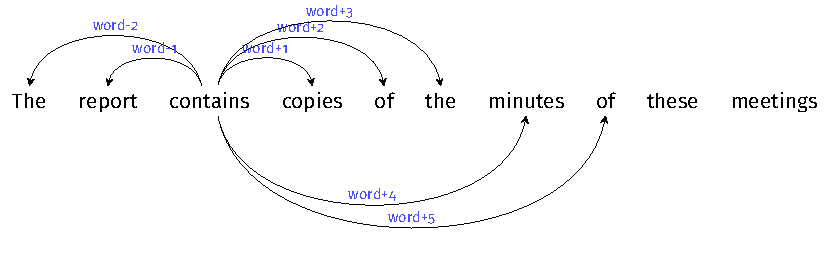
\includegraphics[width=.8\linewidth]{img/tree/lexical_tree.pdf}
  \onslide<10>
%	  \textbf{Dependency Information}  
  	  
  	  \centering
      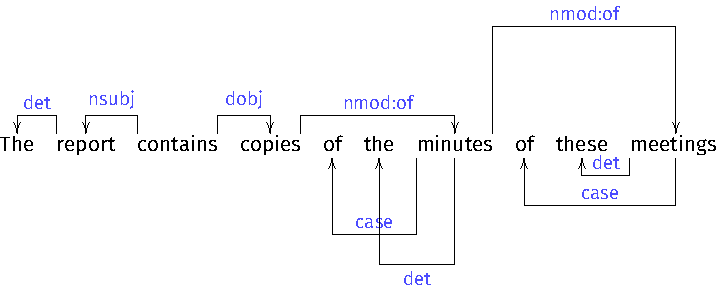
\includegraphics[width=.8\linewidth]{img/tree/dep_tree.pdf}
  \onslide<9>
%	  \textbf{Constituency Information}  
	  
	  \centering
      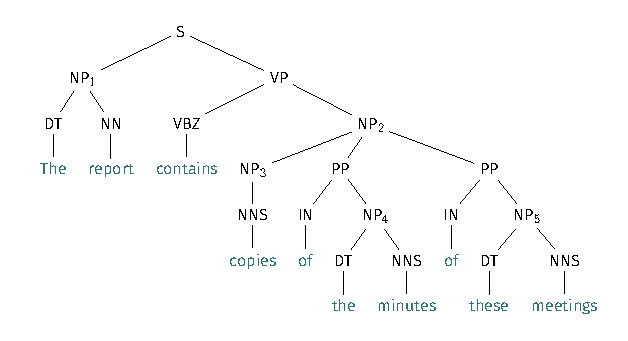
\includegraphics[width=.8\linewidth]{img/tree/tree.pdf}
\end{overprint}

%boilerplate
%\begin{overprint}
%  % on every slide (not sure if it is officially supported)
%  \onslide<1>
%  % on first slide
%  \onslide<2>
%  % on slide two
%  \onslide<3>
%  % on slide three
%  % etc.
%\end{overprint}

\end{frame}

\begin{frame}{Representing Text}
\begin{itemize}
\item \textbf{Text Representation Models}
	\begin{itemize}
		\item Words and features can be represented by means of graph-based models  matrices
		\item Or directly with (sparse) matrices
	\end{itemize}
\item \textbf{Leveraging the Network Structure}
	\begin{itemize}
		\item We can find communities of similiar words according to their meaning
	\end{itemize}
\end{itemize}
\begin{overprint}
	  % on every slide (not sure if it is officially supported)
	  \onslide<2>
	  \centering
	      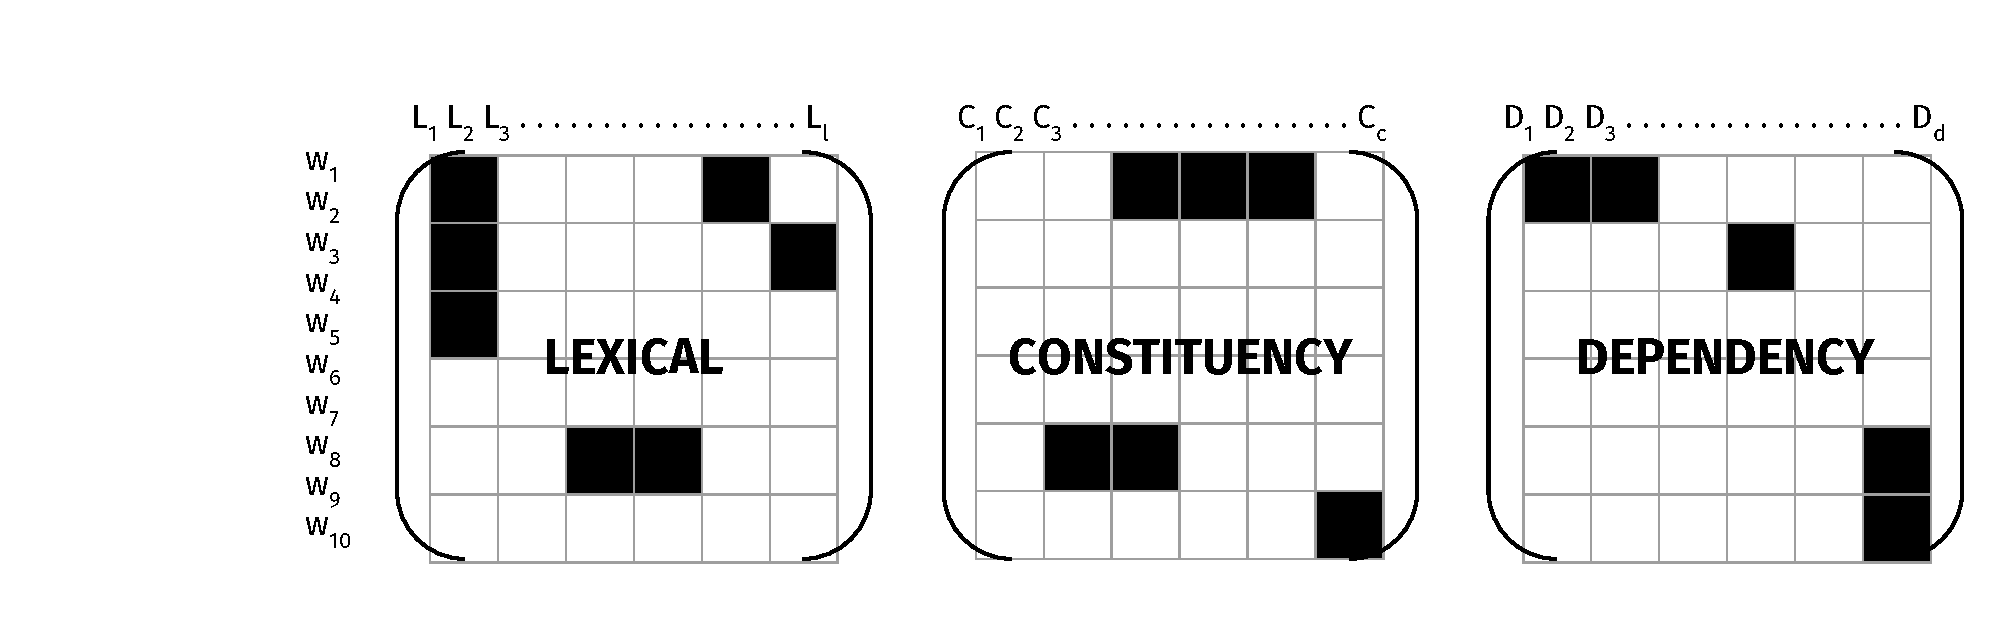
\includegraphics[width=.8\linewidth]{image2/Chapitre1/feature_types.pdf}	
%	  \onslide<3>
%	  \centering
%		  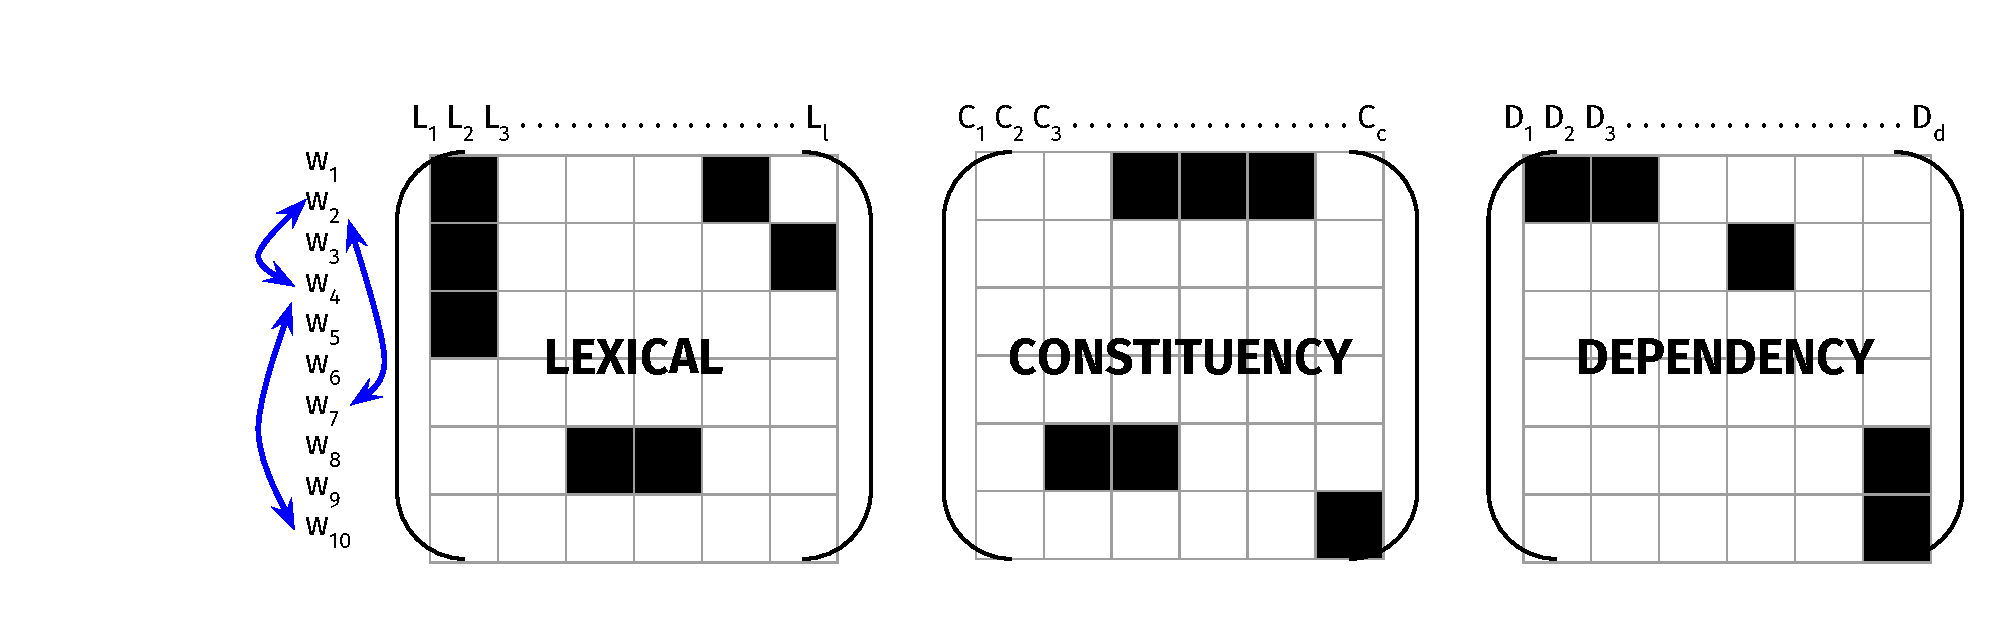
\includegraphics[width=\linewidth]{image2/Chapitre1/feature_types_communities.pdf}	  
	  % on slide two
\end{overprint}

\end{frame}


\begin{frame}{Main Challenges and Contributions}
	\begin{enumerate}[<+- | alert@+>]
		\item What type of model can we employ to represent a corpus using heterogeneous features?
		%    	    	 what type of model can we employ to represent a corpus through a set of heterogeneous features, extracted from itself, while keeping record of the relationships between textual units? How can we organize and store this model as simply and efficiently possible?
		\begin{itemize}
		\item \textit{Hypergraph linguistic model to hold different types of  linguistic information}
		\end{itemize}
		
		\item How can we combine these features while dealing with feature sparsity?
		\begin{itemize}
		\item \textit{Multimedia fusion techniques to combine and densify representation spaces}	    	 
		\end{itemize}
		\item How can we find and employ communities existing within the language networks?
		\begin{itemize}
		\item \textit{An alternative network-based algorithm to discover semantically related words within a text}
		\end{itemize}
		
	\end{enumerate}%[<+- | alert@+>]
 \vspace{\textheight}
\end{frame}


\begin{frame}{Work Overview}
\begin{center}
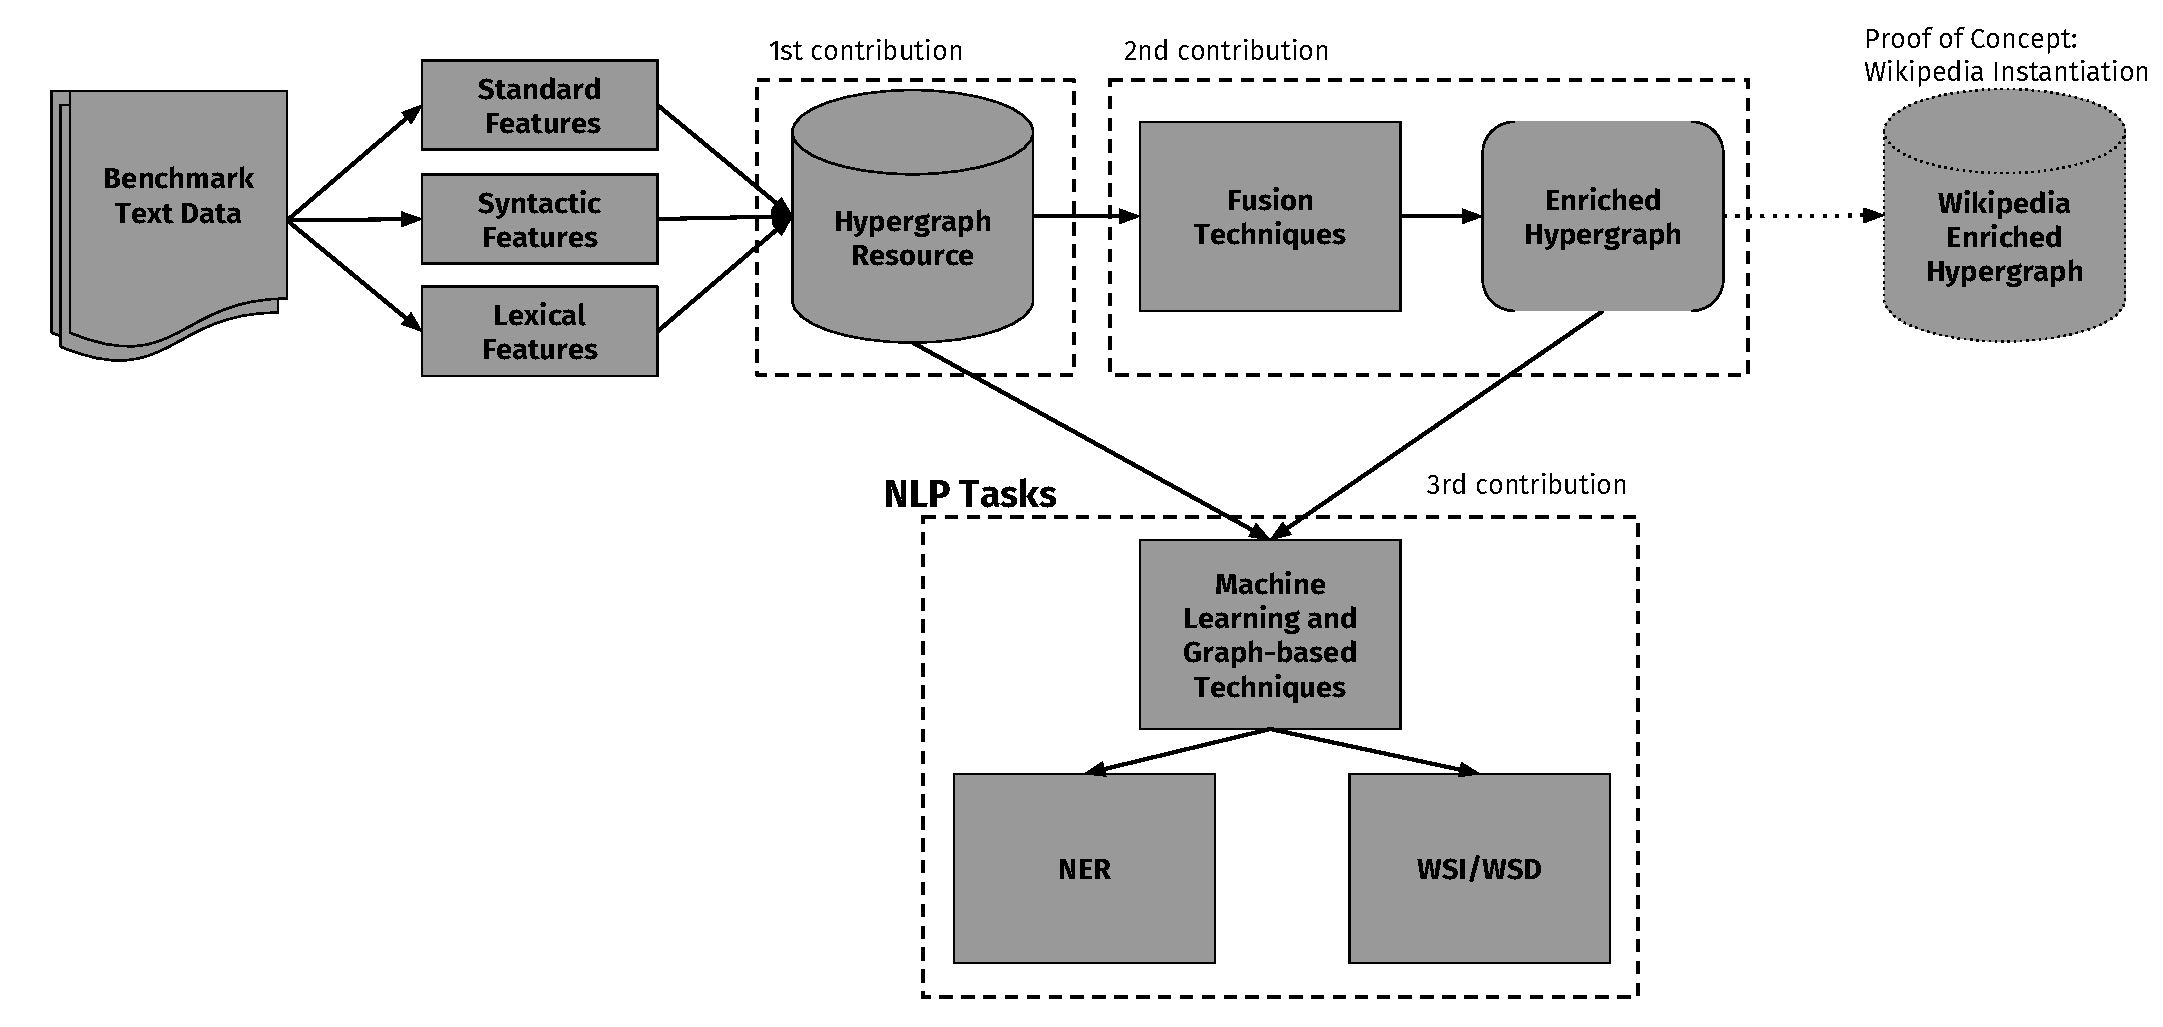
\includegraphics[width=1.04\linewidth]{image2/Chapitre1/main_diag_presi.pdf}
\end{center}

 \vspace{\textheight}
\end{frame}

\setbeamertemplate{section page}[mytheme]

\section[Contributions in Detail]{Hypergraph Linguistic Model}
\metroset{sectionpage=none}
\section{Hypergraph Linguistic Model}
\metroset{sectionpage=simple}
%\begin{frame}{Work Overview}
%%\large  \textbf{Approach Overview} \hfill
%\begin{center}
%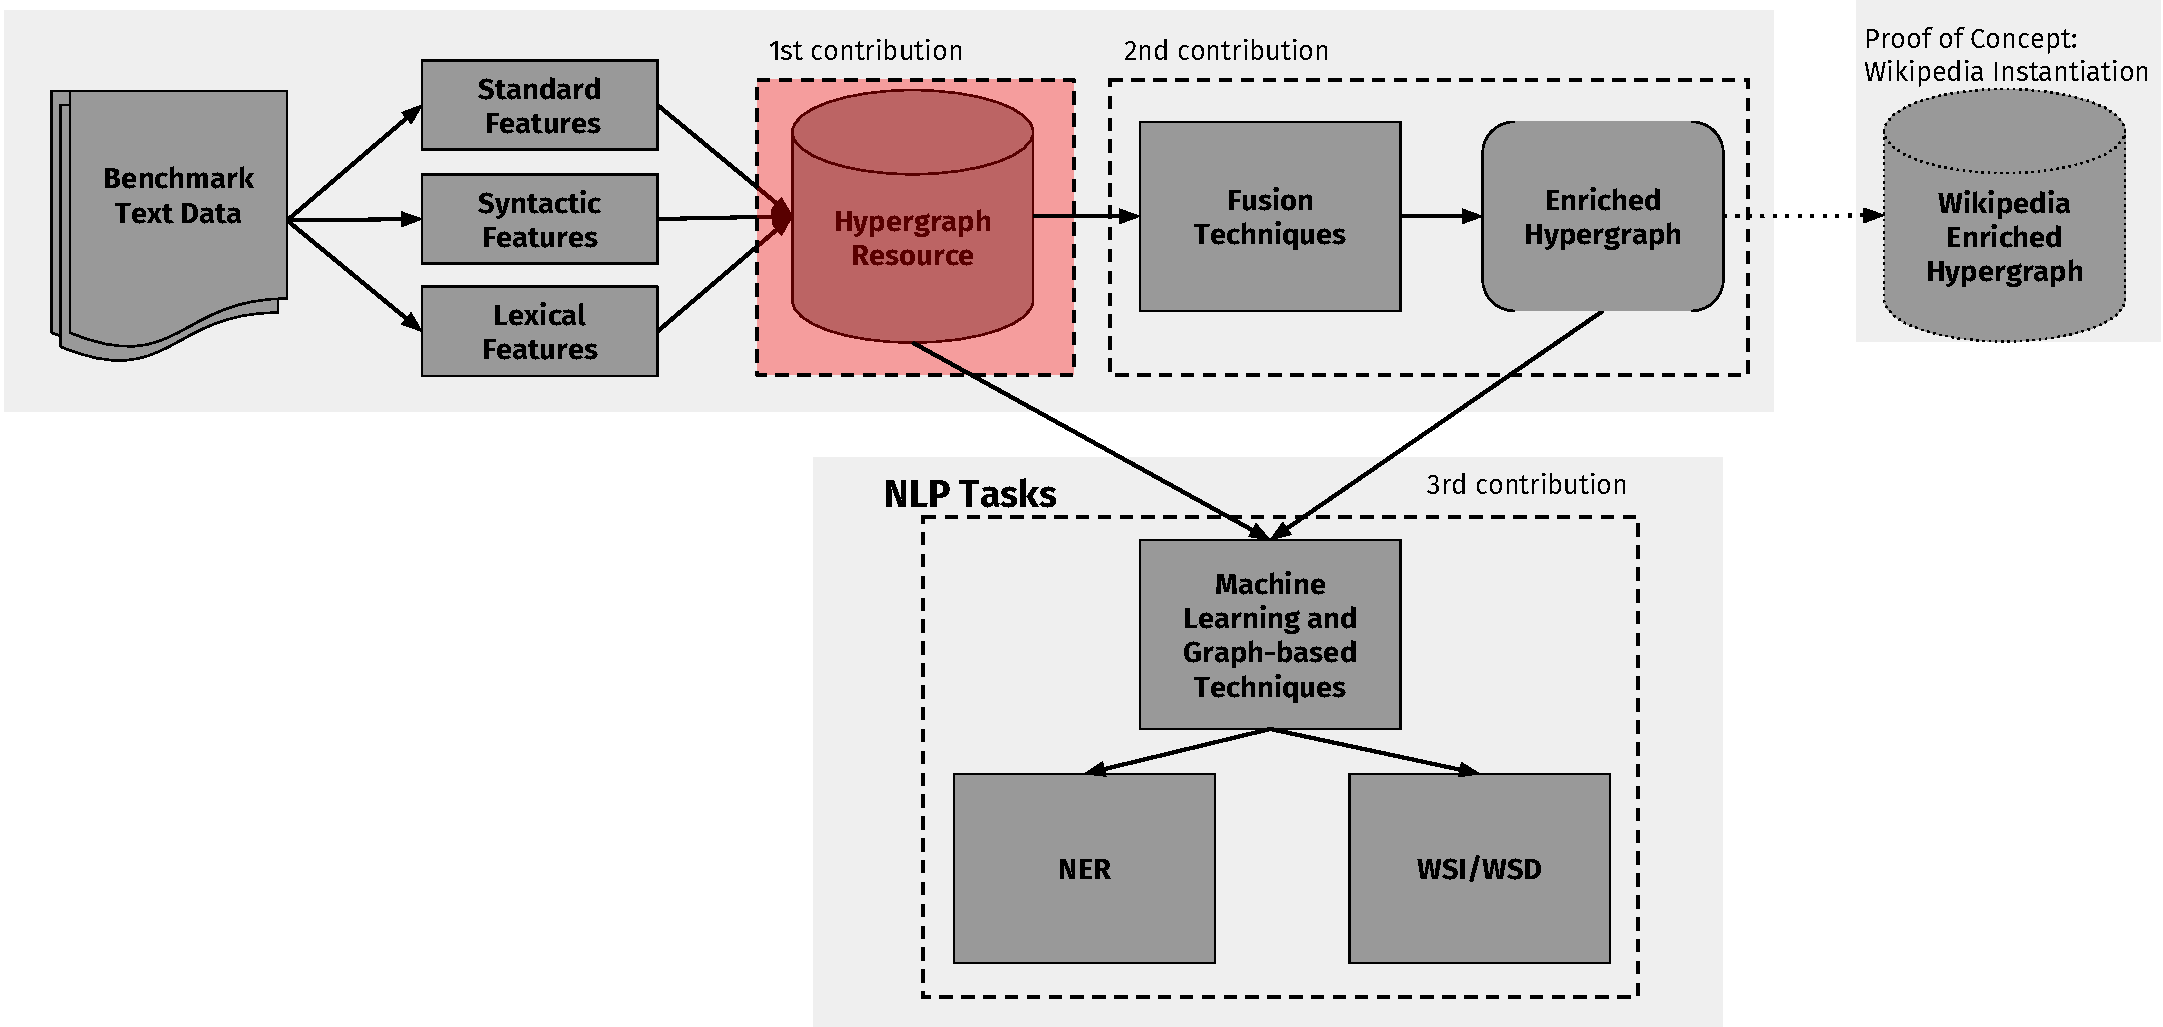
\includegraphics[width=1.04\linewidth]{image2/Chapitre3/main_diag_contr1.pdf}
%\end{center}
%
% \vspace{\textheight}
%\end{frame} 


\begin{frame}{Introduction}
%\large \textbf{What type of model can we employ to represent textual features?}
%Which textual features?
%todo Add here the networks by choudhury et al, venus stuff
\vspace{.5cm}
Based on the distributional hypothesis, a word is defined by its surroundings, we can extract useful information from a text.
\begin{itemize}[<+- | alert@+>]
	\item \textbf{How do we represent textual data?}
		\begin{itemize}
		\item Network Models \cite{2004.Mihalcea.SemanticNetworkPageRank}
		\item Vector Space Models \cite{manning1999foundations}

		
		\end{itemize}
	\vspace{.5cm}
	\item \textbf{We choose network models} 
		\begin{itemize}
		\item Used in a large quantity of NLP tasks \cite{Mihalcea2011}
		\item Graphs structures can give us a clearer view into the relations of words within a text 	\cite{Choudhury2009}
		\item Ultimately graphs are transformed to a vectorial representation through the adjacency/incidence matrices
		
		\end{itemize}
		
\end{itemize}
\vspace{\textheight}
\end{frame}




\begin{frame}{Classic Language Networks}
%What is the state of the art ? How is text is represented by means of networks?
% Three main types
%todo Add here the networks by choudhury et al venus stuff

\begin{itemize}
\item[] \textit{The report contains copies of the minutes of these meetings} 
\end{itemize}

\begin{overprint}
  % on every slide (not sure if it is officially supported)
  \onslide<2>
	  \centering
	  
	  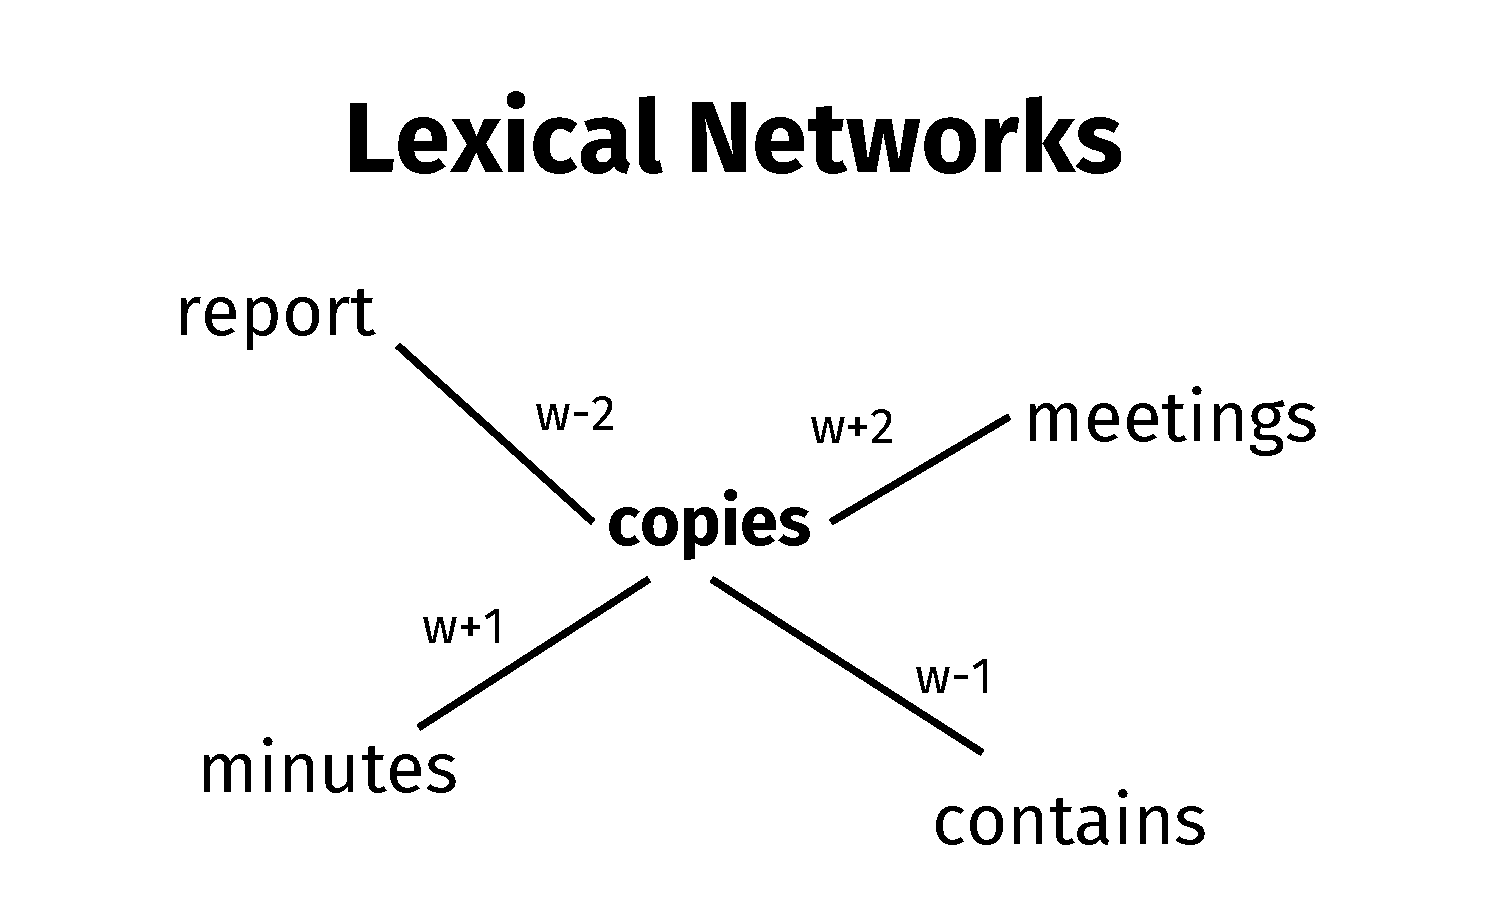
\includegraphics[width=.7\linewidth]{image2/Chapitre2/lexi_network_ex.pdf}
	  \\ \cite{2008.Klapaftis.WSIUsingCollocations}
  \onslide<3>
	  \centering
	  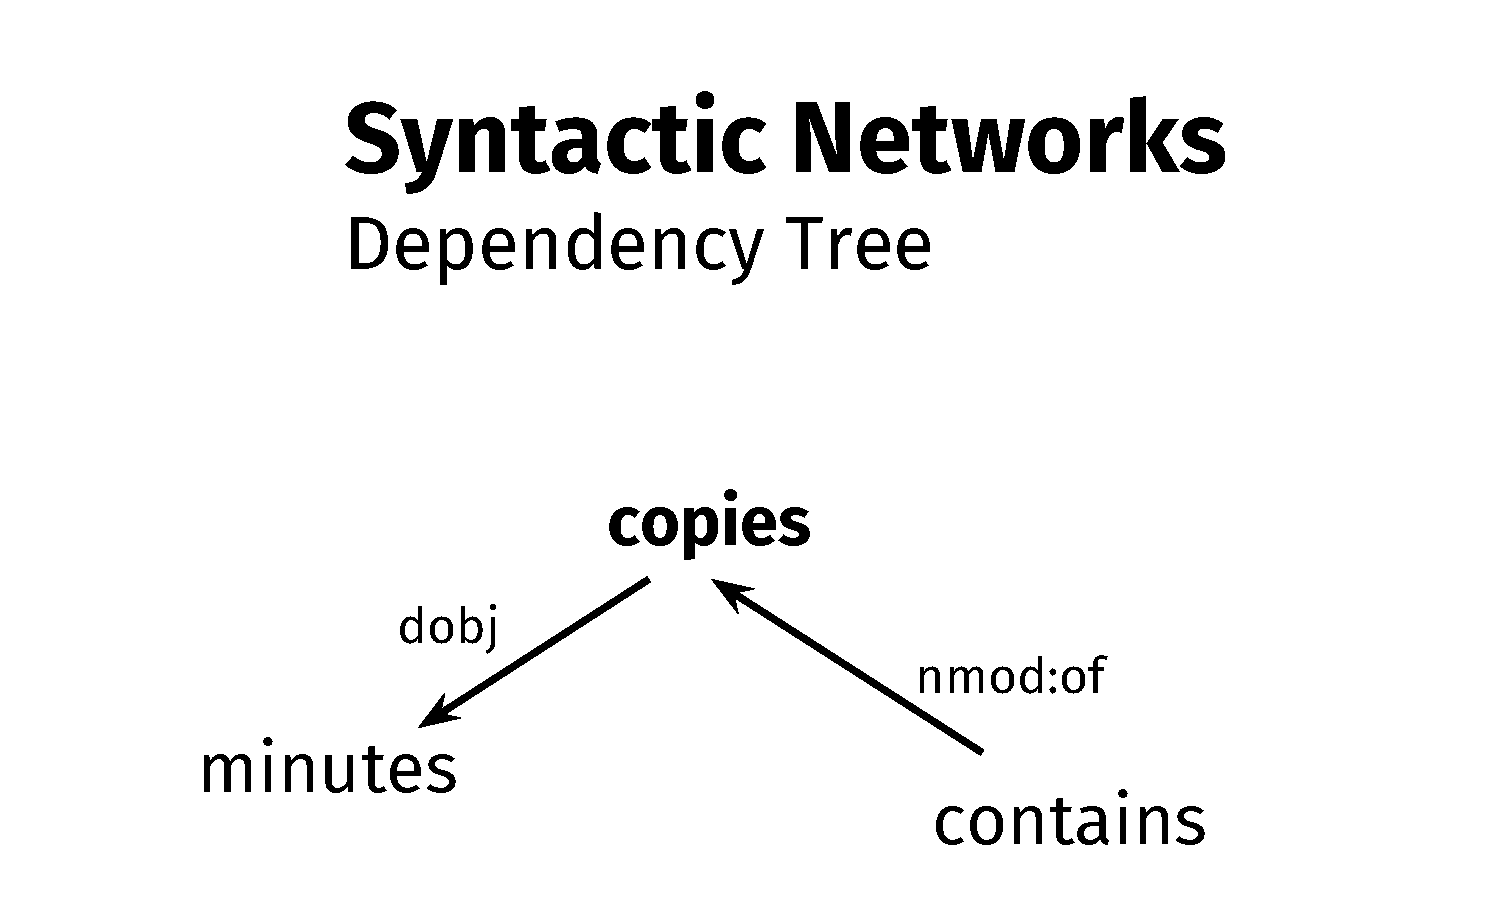
\includegraphics[width=.7\linewidth]{image2/Chapitre2/deps_network_ex.pdf} 
  \onslide<4>
	  \centering
	  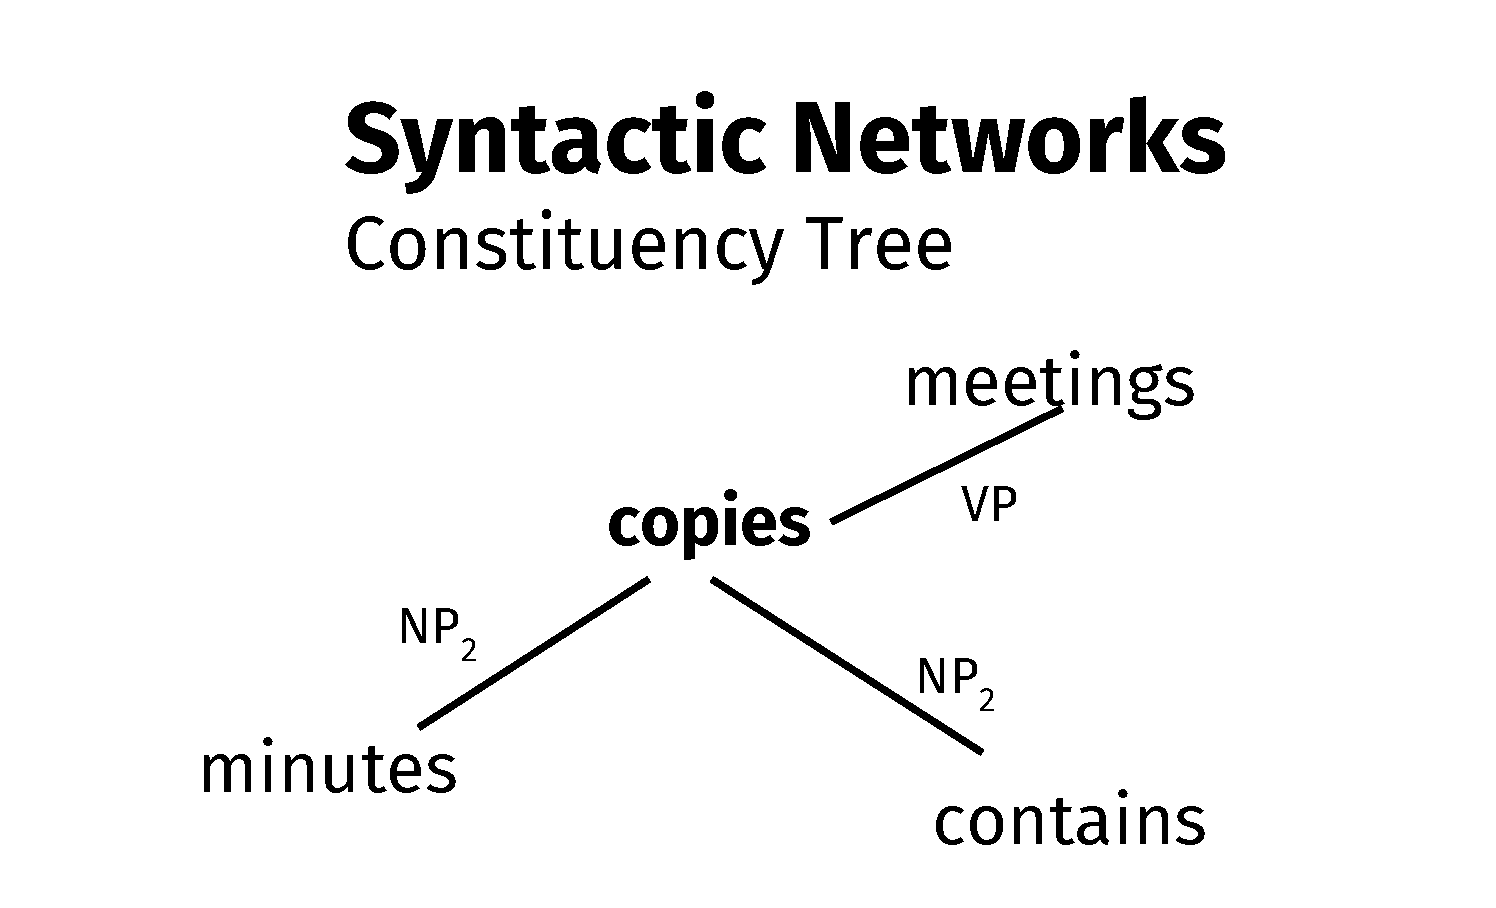
\includegraphics[width=.7\linewidth]{image2/Chapitre2/consti_network_ex.pdf}   
  \onslide<5>
	  \centering
	  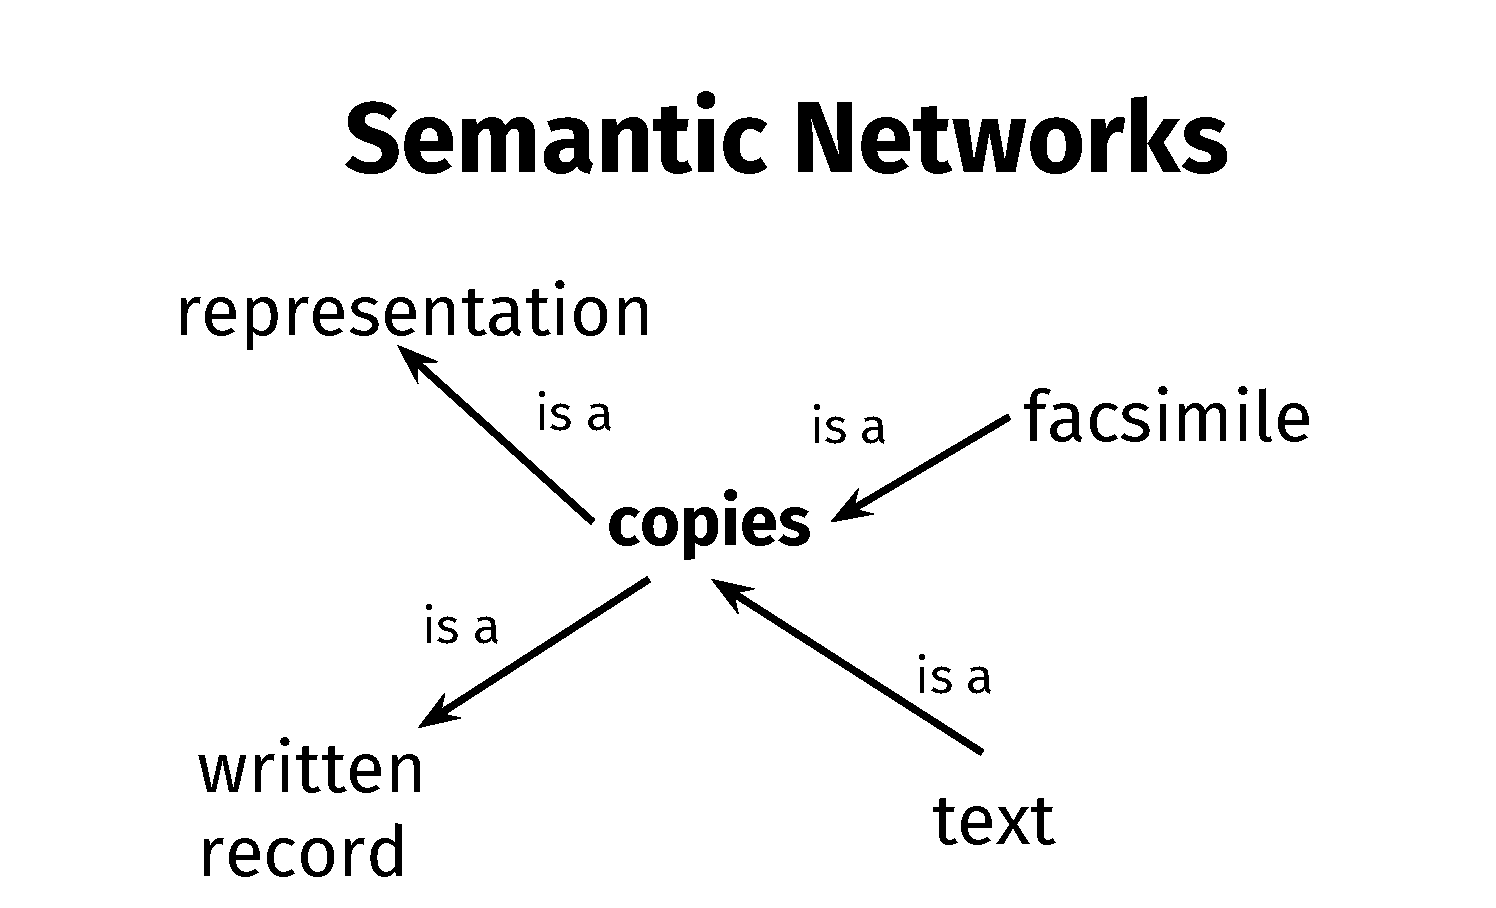
\includegraphics[width=.7\linewidth]{image2/Chapitre2/sem_network_ex.pdf}   

  % on slide three
  % etc.
\end{overprint}



%\begin{columns}
%	\column{0.33\textwidth}
%	\centering
%	\onslide<3->\textbf{Lexical Networks}
%	\begin{minipage}[c][0.6\textheight][c]{\linewidth}
%	\onslide<4->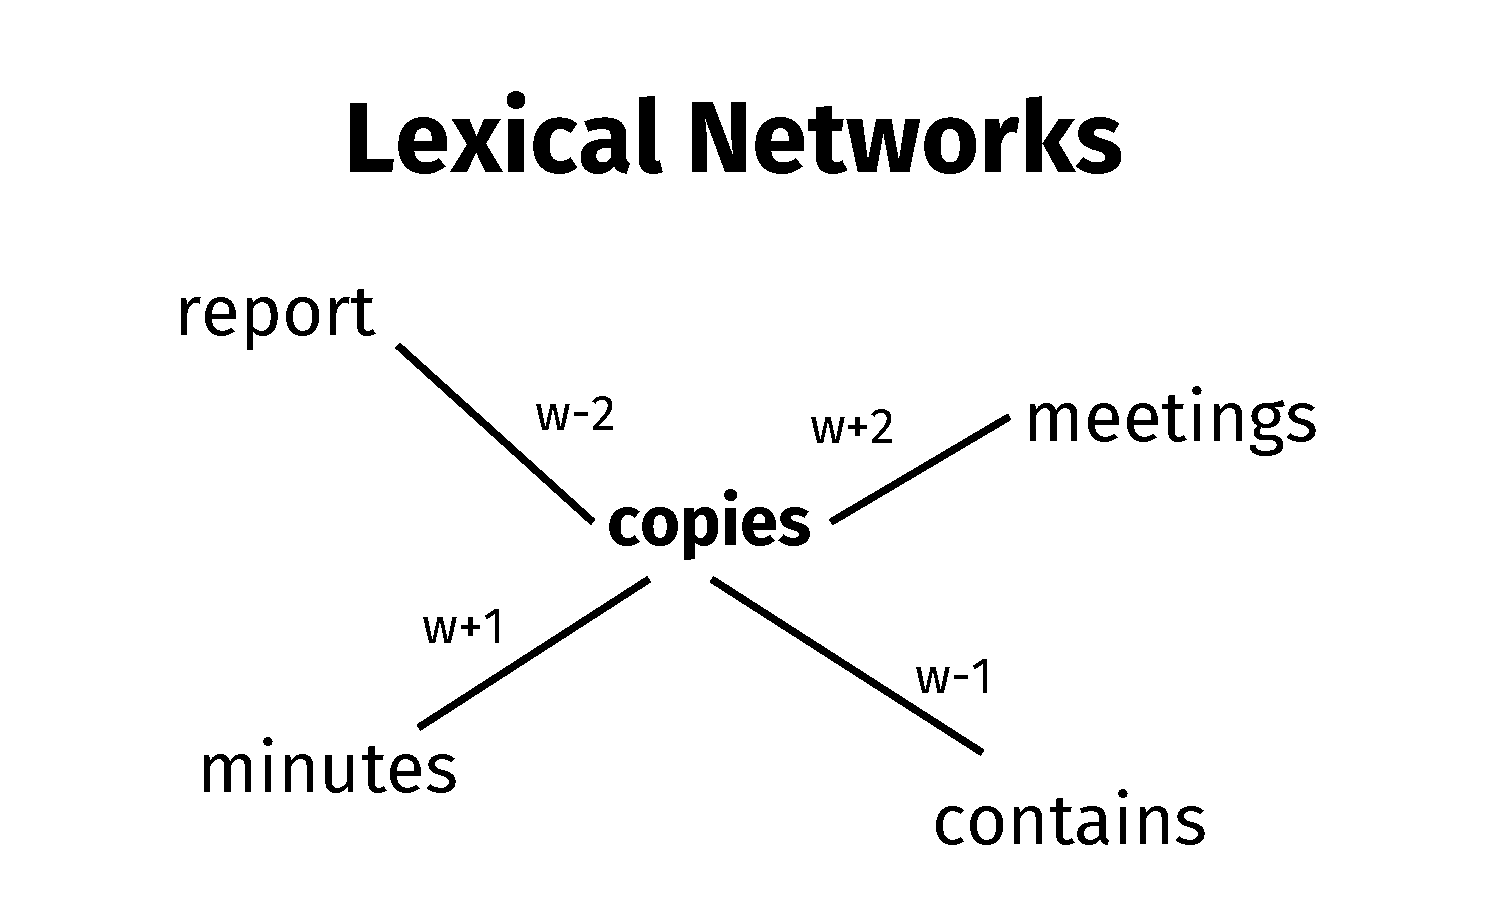
\includegraphics[width=1\linewidth]{image2/Chapitre2/lexi_network_ex.pdf}
%	\end{minipage}
%	\column{0.33\textwidth}
%	\centering
%	\onslide<5->\textbf{\normalsize Syntactic Network} 
%	\begin{minipage}[c][0.6\textheight][c]{\linewidth}
%	\onslide<6->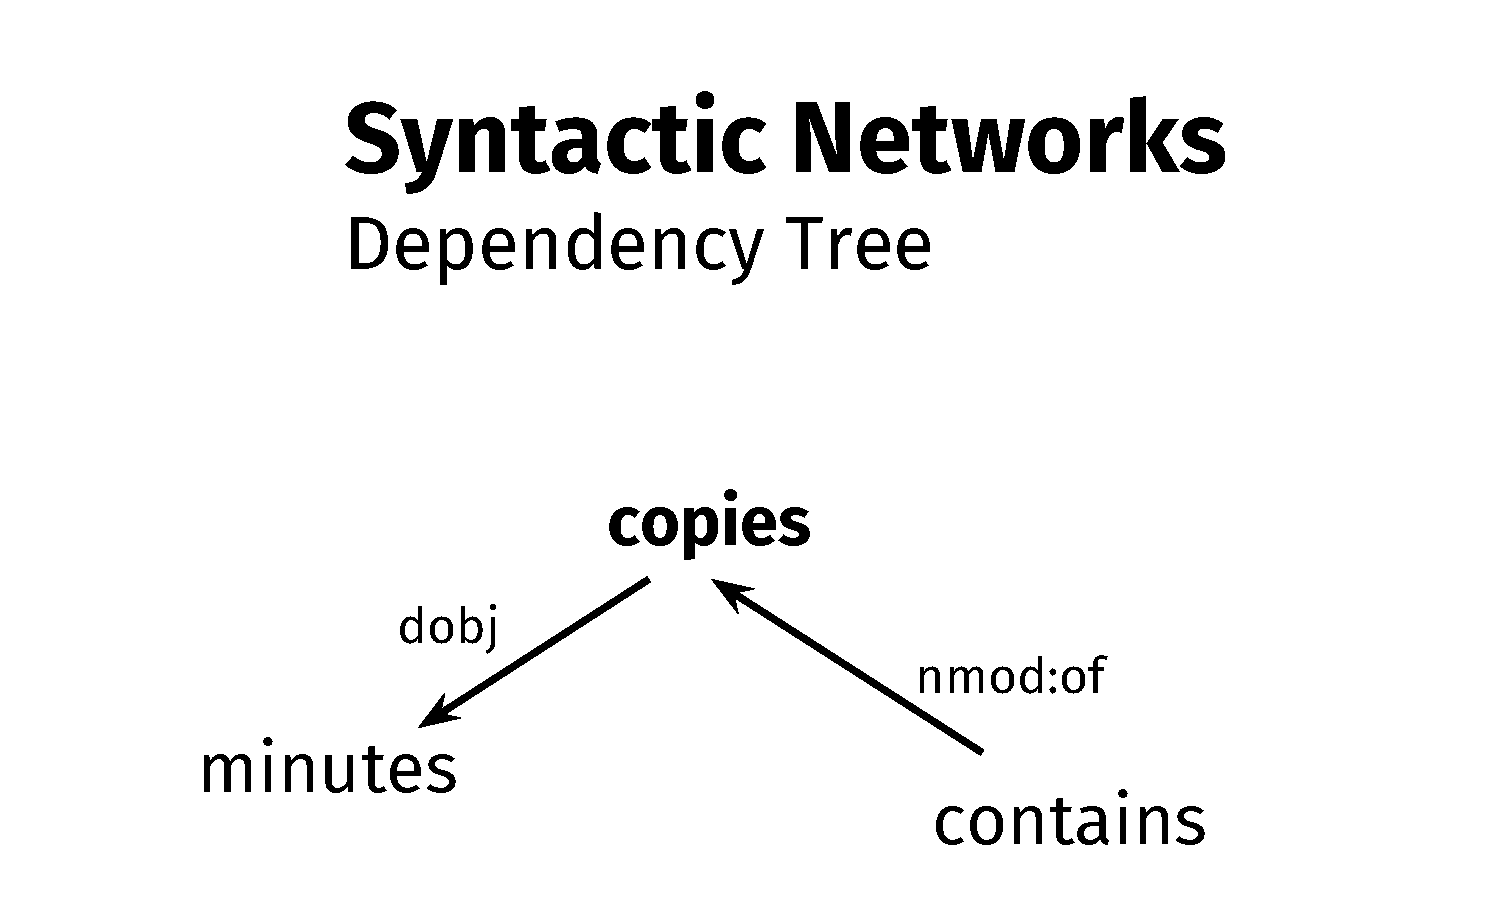
\includegraphics[width=1\linewidth]{image2/Chapitre2/deps_network_ex.pdf} \\
%	\onslide<7->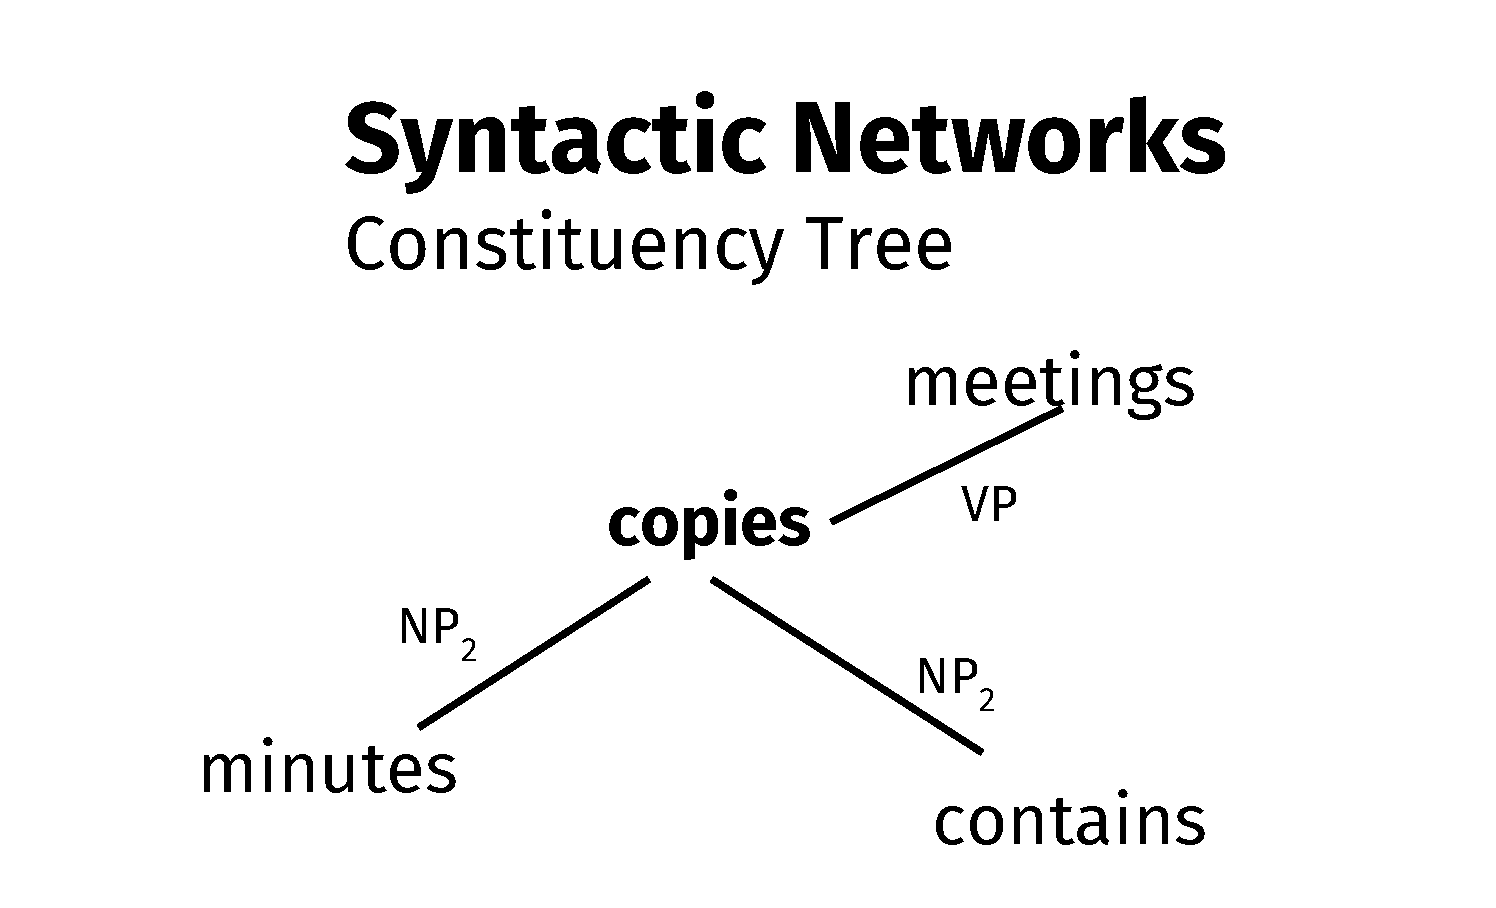
\includegraphics[width=1\linewidth]{image2/Chapitre2/consti_network_ex.pdf}
%	\end{minipage}
%	
%	\column{0.32\textwidth}
%	\onslide<8->\textbf{\normalsize Semantic Network} 
%	\begin{minipage}[c][0.6\textheight][c]{\linewidth}
%	\onslide<9->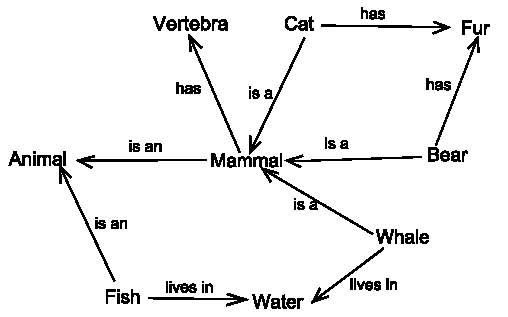
\includegraphics[width=1\linewidth]{image2/Chapitre2/sem_net.pdf}
%	An expert is usually involved.
%	\end{minipage}
%
%\end{columns}

\end{frame}


\begin{frame}{Limitations and Proposition}
\begin{itemize}[<+- | alert@+>]
\item \large \textbf{Limitations of existing representations}
	\begin{itemize}
	\item Language networks generally employ a single type of textual information
	\item The edges of the network may relate maximum two words at each time
%	\item There is no 
	\end{itemize}
\item \large \textbf{Proposition}
	\begin{itemize}
	\item Represent together linguistic co-occurrences through a hypergraph model
	\begin{itemize}
	\item Link together three different types of networks, using lexical and syntactic data
	\item Get a semantic overview at three different levels: short range (with dependency functions), medium range (phrase constituency membership), and long range (lexical  co-occurrence) 
	\end{itemize}
	
	\end{itemize}
\end{itemize}
\vspace{\textheight}
\end{frame}

%\begin{frame}{Proposed Model: Definitions}
%\large \textbf{Hypergraph Linguistic Model}
%\begin{itemize}
%	
%	\item \textbf{Hypergraph:}
%	\begin{itemize}
%		\item A graph generalization, where edges may link more than 2 nodes at the same time. It can be seen as a set of sets
%	\end{itemize}
%
%\end{itemize}
%\centering
%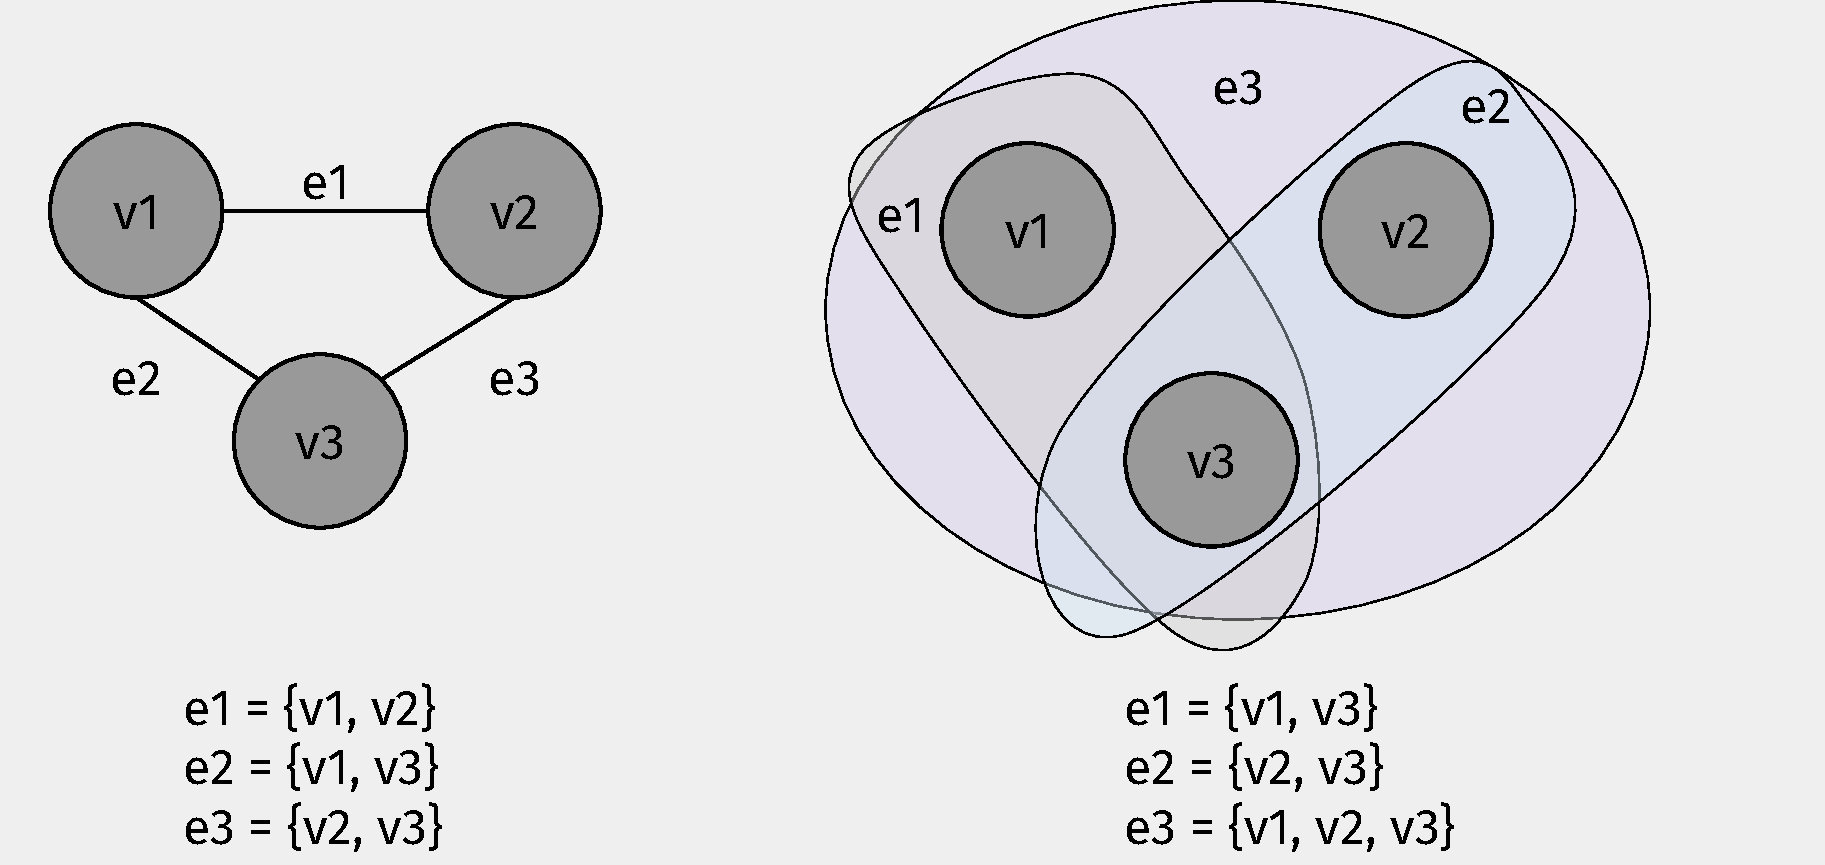
\includegraphics[width=1\linewidth]{image2/Chapitre3/graph_vs_hgraph.pdf}
%\vspace{\textheight}
%\end{frame}


%\begin{frame}{Proposed Model: Definitions}
%\large \textbf{Hypergraph Linguistic Model}
%\begin{itemize}
%	
%	\item \textbf{Linguistic Features:}
%	\begin{enumerate}
%		\item \textbf{CONSTITUENT $\mathbf{(M^N)}$:} noun phrase constituents memberships
%		\item \textbf{DEPENDENCY $\mathbf{(M^S)}$} dependency relations. We consider all types of dependency functions between nouns and verbs,
%		\item \textbf{SENTENCE $\mathbf{(M^L)}$:} lexical context, in this case the window considered is the whole sentence
%	\end{enumerate}
%	\item **Show image with the three different levels**
%\end{itemize}
%\centering
%\vspace{\textheight}
%\end{frame}



%\begin{frame}{Proposed Model: Working Example}
%\begin{itemize}
%	\item \large \textbf{Input:} Set of linguistic features from an entry corpus
%	\item \textbf{Output:} A network relating words according to the input features. Computationally, a key-value structure holding words and their descriptors for fast retrieval
%	\item   \textbf{Example sentence \textbf{S$_1$}:}
%		\begin{itemize}
%			\item[]  \textit{The report contains \textbf{copies} of the minutes of these meetings}. \note{After tokenization,  lemmatization and parsing, we obtain both constituency and dependency trees.}
%		\end{itemize}
%	
%	 
%\end{itemize}
%
%\begin{columns}
%	\column{0.7\textwidth}
%	\begin{minipage}[c][0.4\textheight][c]{\linewidth}
%	\centering
%	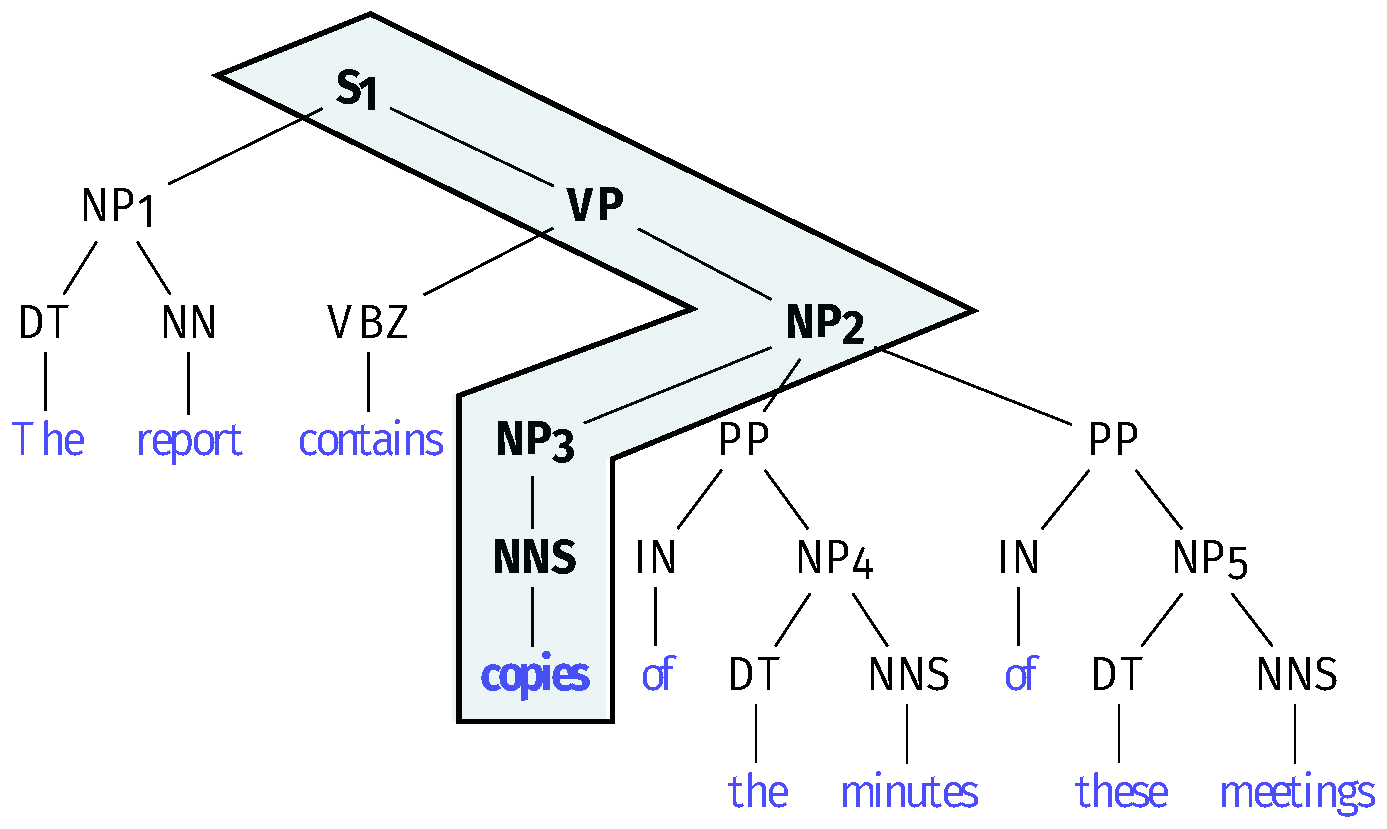
\includegraphics[width=.8\linewidth]{img/tree.pdf}
%	\end{minipage}
%	\column{0.35\textwidth}
%	\begin{minipage}[c][0.4\textheight][c]{\linewidth}
%	%  \centering
%	%\large
%	\color{black!40}root(root,~contains) \\
%	\color{black!40}det(report,~The) \\
%	\color{blue!70}{\textbf{dobj(contains,~copies)}}
%	\color{black!40}case(minutes,~of)
%	\end{minipage}
%\end{columns}
%
%\end{frame}


\begin{frame}{Proposed Model}
	\begin{itemize}
		\item Explain (grpahically/with the working exampleh) we use lexical and syntactic info and the build a fusion of them with a hypergraph.
	\end{itemize}

	\begin{columns}
		\column{1\textwidth}
		\begin{minipage}[c][0.4\textheight][c]{\linewidth}
			 \centering
			 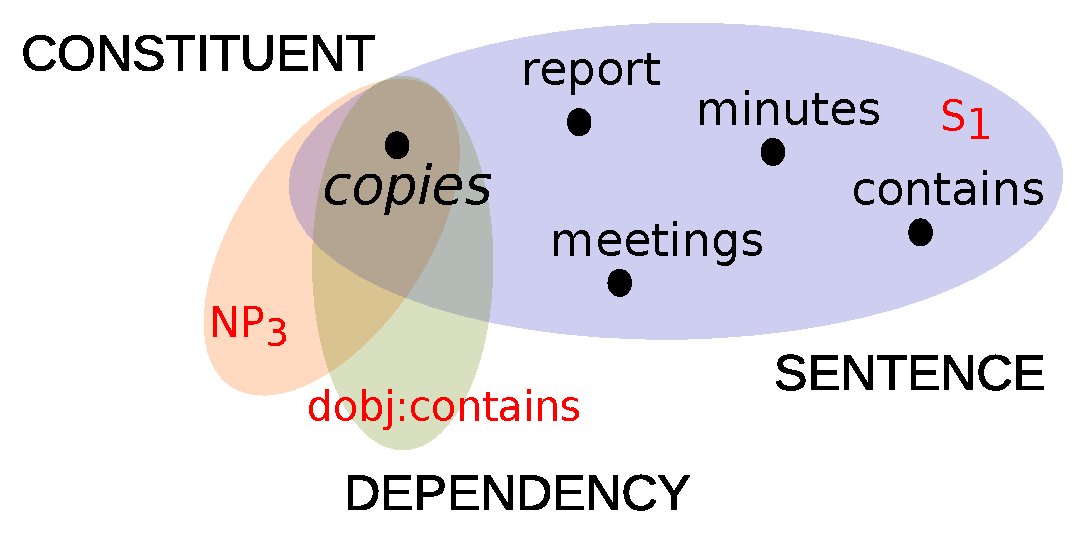
\includegraphics[width=.6\linewidth]{img/hypergraph_copies.pdf} <===== THIS!
		\end{minipage}
		\begin{minipage}[c][0.5\textheight][c]{\linewidth}
			\centering
			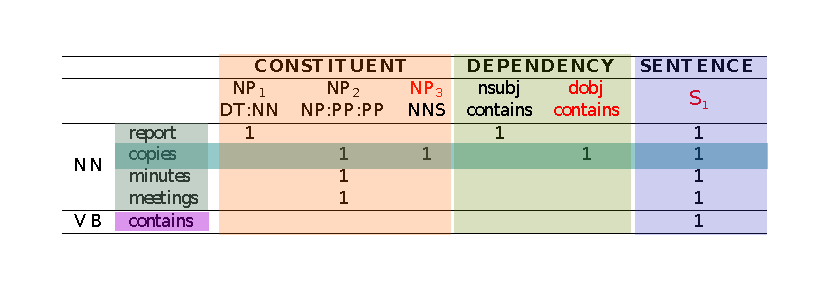
\includegraphics[width=.9\linewidth]{img/incidence_aug.pdf}
		\end{minipage}
	\end{columns}
\end{frame}



\setbeamertemplate{section page}[mytheme]
\section[Contributions in Detail]{Combining Features and Dealing with Sparsity}                  

      
\begin{frame}{Introduction}
\large \textbf{Multimedia Fusion Techniques \cite{AtreyHEK10,ahn2010link}}:
%\vspace{.5cm}
\begin{itemize}
\item \large \textbf{Definition}
	\begin{itemize}
	\item Set of techniques used in multimedia analysis tasks to integrate multiple media 
	\item The goal is to obtain rich insights about the data being treated
	\item We adapt these techniques to our use case: textual information
	\end{itemize}
\item \textbf{Main fusion operators:}
	\begin{itemize}
	\item Early Fusion $E_\alpha(\cdot)$, 
	\item Late Fusion $L_\beta(\cdot)$, 
	\item Cross Fusion $X_\gamma(\cdot), X_F(\cdot)$
	\item $\alpha$ and $\beta$: Assign an importance weight to each of their operators 
	\item $\gamma$: number of top similar items to take from the similarity space
	\end{itemize}

\end{itemize}
\end{frame}




\begin{frame}{Early and Late Fusion}
\begin{center}
\end{center}
\begin{columns}
	\column{0.5\textwidth}
	\begin{minipage}[c][0.5\textheight][c]{\linewidth}
		\centering
		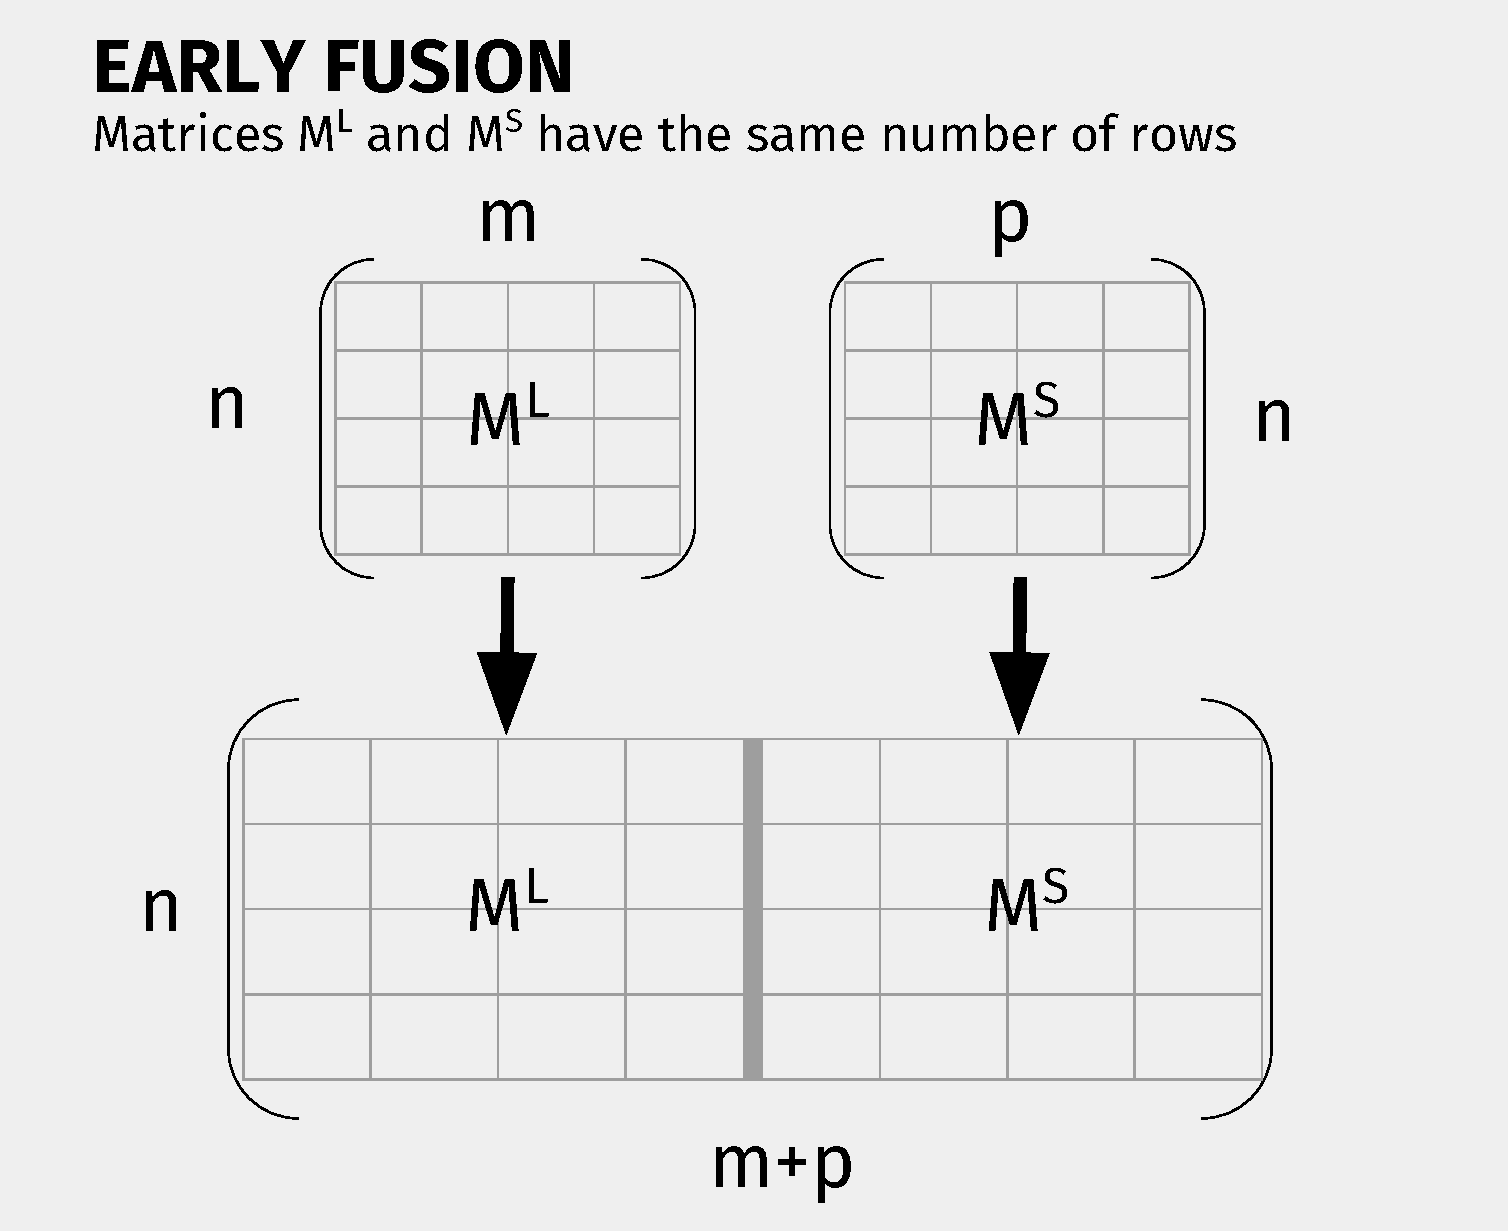
\includegraphics[width=1\linewidth]{image2/Chapitre3/ef_diag}
		\end{minipage}
		\column{0.5\textwidth}
	\begin{minipage}[c][0.5\textheight][c]{\linewidth}
		\centering
	  	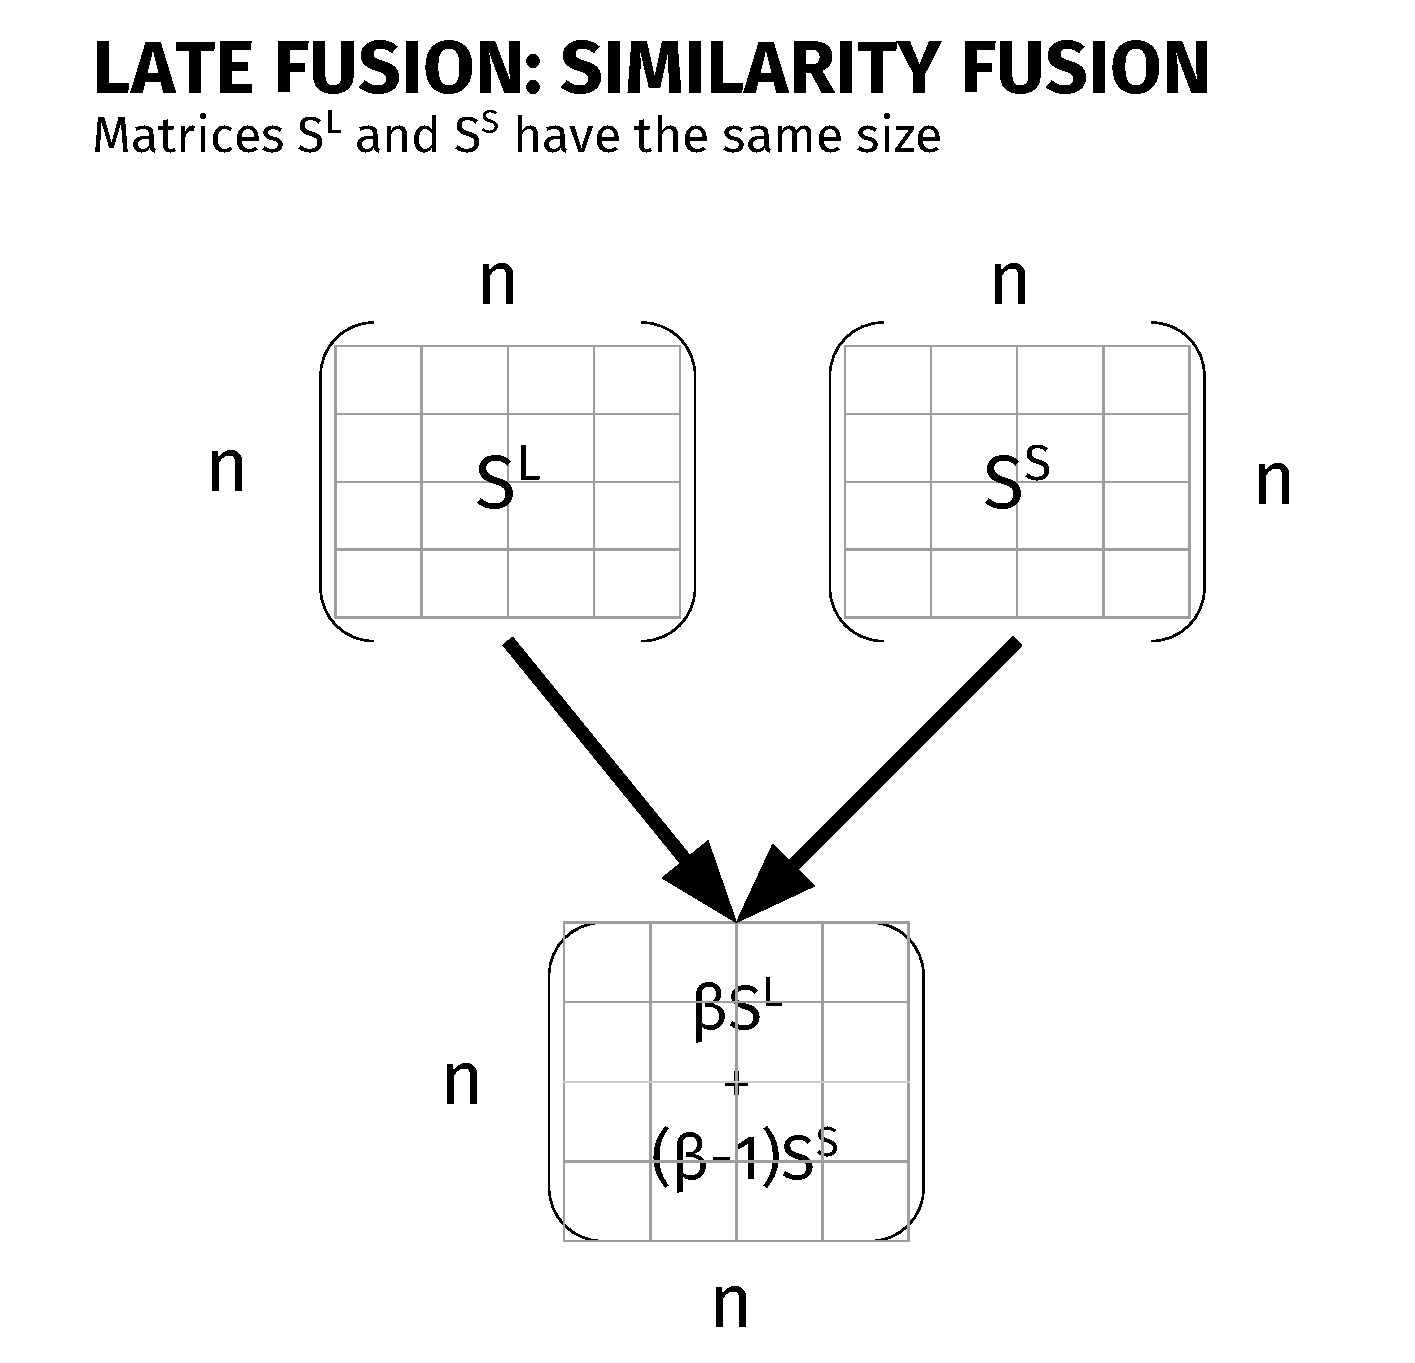
\includegraphics[width=1\linewidth]{image2/Chapitre3/lf2_diag.pdf}
	\end{minipage}
\end{columns}




\end{frame}



\begin{frame}{Cross Fusion}
\begin{center}
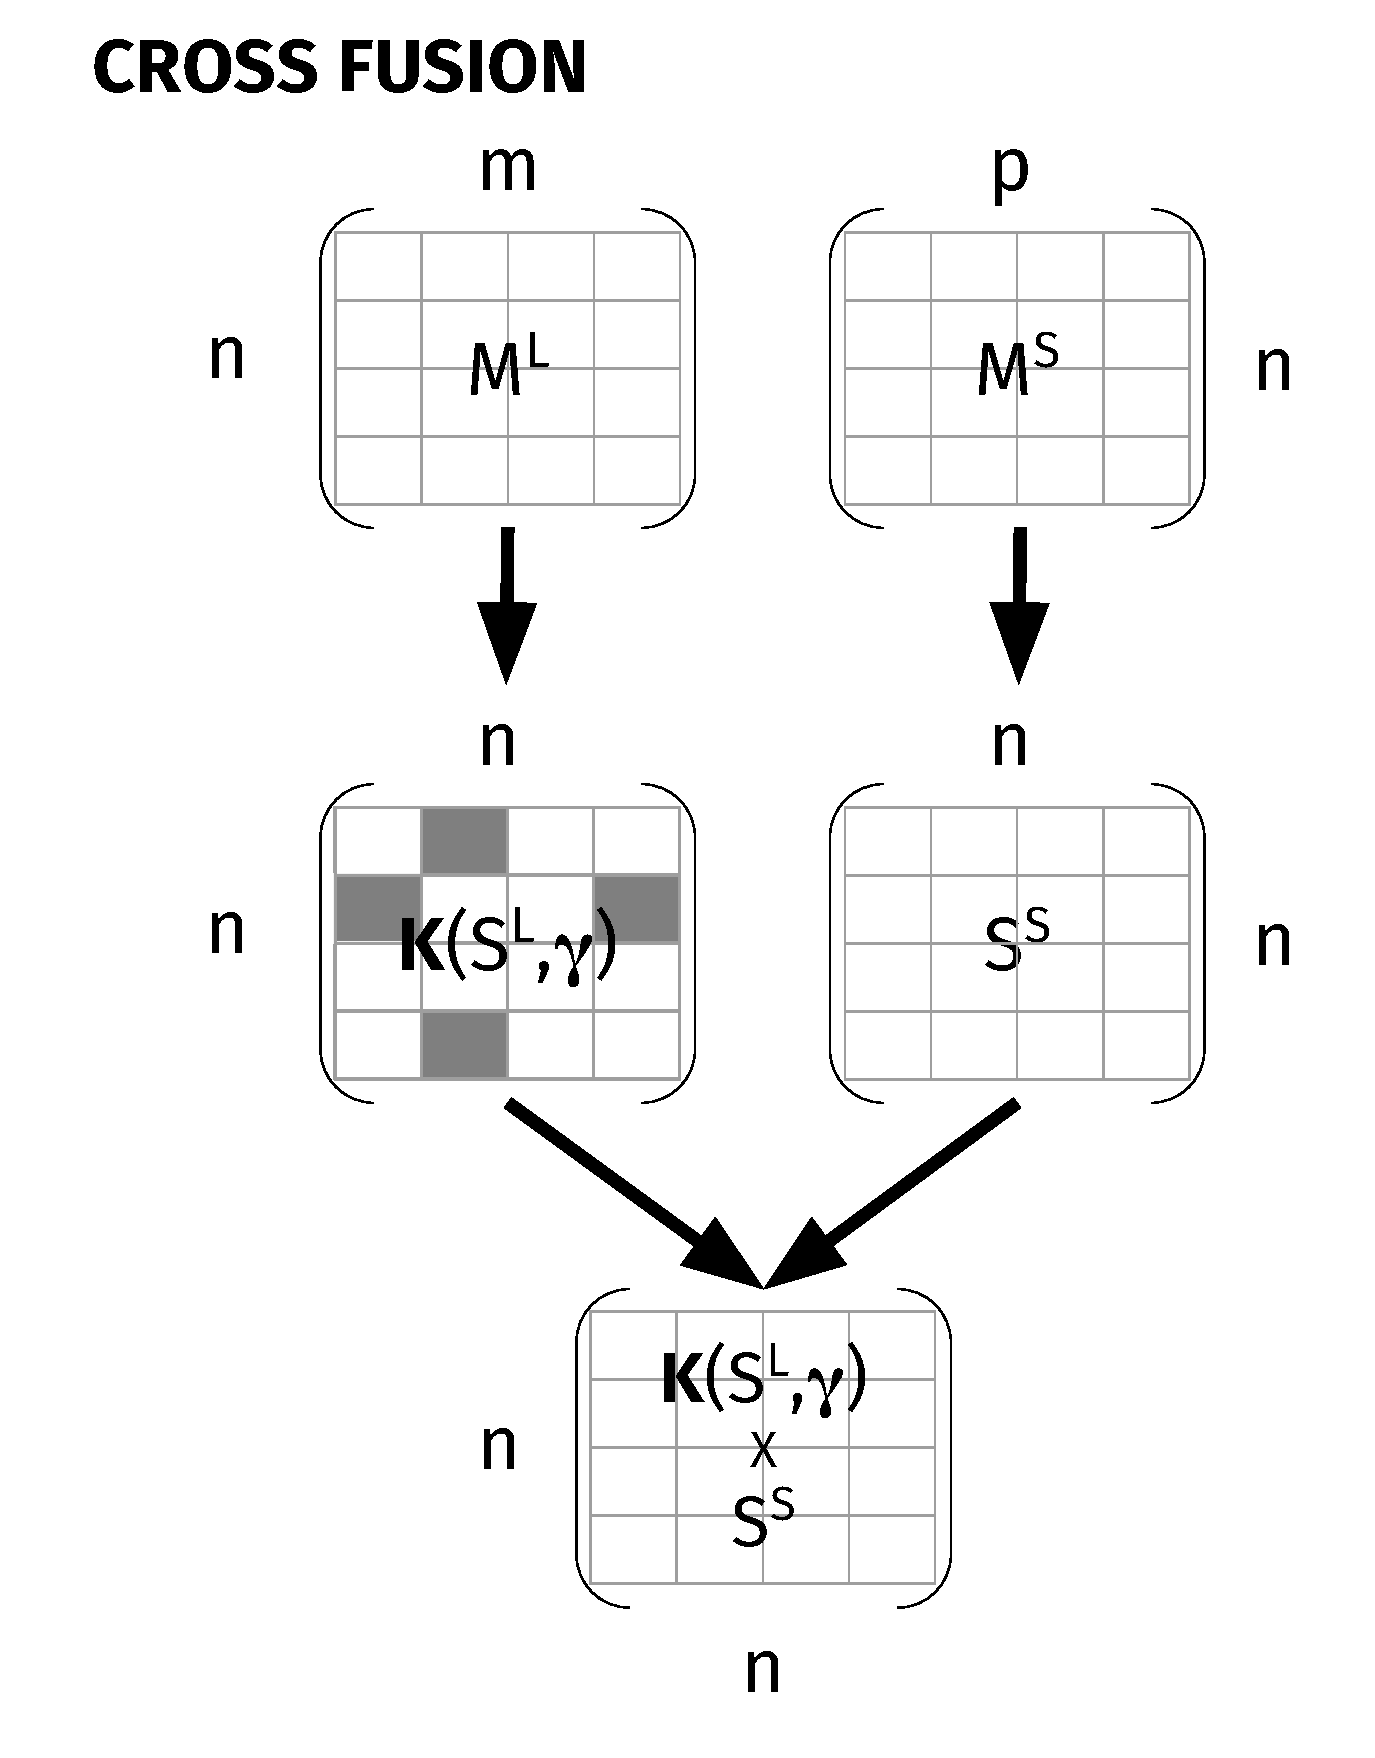
\includegraphics[width=.55\linewidth]{image2/Chapitre3/xf_diag.pdf}
\end{center}
\end{frame}


\begin{frame}{Hybrid Fusion 1}
\begin{itemize}
\item [] \large Put here some very visual way of representing hybrid fusion.
\item [] In fact, early and late fusion should be presented with the working example also.
\end{itemize}

\end{frame}

\begin{frame}{Hybrid Fusion 2}
\begin{itemize}
\item [] \large Put here some very visual way of representing hybrid fusion.
\item [] In fact, early and late fusion should be presented with the working example also.
\end{itemize}

\end{frame}




\begin{frame}{Leveraging the network communities}
\begin{enumerate}
\item  Show a large (with more text than that of my example) image of  the hypergraph model


\end{enumerate}
\end{frame}

\section[Contributions in Detail]{Finding Communities in the Network}

\begin{frame}{Leveraging the network communities 1}
\begin{enumerate}
\item Link some words together with a color overlay to represent possible communities (clusters/groups) of same sense words. 
\item Argue that thanks to the heterogeneous info contained in the structure, we can relate words according to different linguistic properties 

\end{enumerate}
\end{frame}

\begin{frame}{Leveraging the network communities 2} 
\begin{enumerate}
\item Link some words together with a color overlay to represent possible communities (clusters/groups) of same sense words. 
\item Argue that thanks to the heterogeneous info contained in the structure, we can relate words according to different linguistic properties 

\end{enumerate}
\end{frame}

\section[Applications to NLP]{Hypergraph Model Instantiation}



\begin{frame}{Introduction}
\large \textbf{Applications}
\vspace{.5cm}
\begin{itemize}
\item We instantiate our proposed linguistic resource 
\begin{itemize}
\item Based on the English Wikipedia corpus
\end{itemize}
\item Use the proposed model  to solve two NLP tasks:
	\begin{itemize}
	\item Named Entity Recognition 
	\item Word Sense Induction and Disambiguation
	\end{itemize}
\vspace{.3cm}
\item These experiments have two main objectives:
	\begin{itemize}
	\item Test the effectiveness of fusion enriched representations (heterogeneity + less sparse spaces)
	\item Leverage the structure of the network built following our proposed model
	\end{itemize}

\end{itemize}
\vspace{\textheight}
\end{frame}

\subsection{Hypergrpah Model Instantiation}
\begin{frame}{Hypergraph Model Instantiation}
\begin{itemize}
\item Introduction to SAEWD
\item Motivation
\item Characteristics
\item Show small diagram of the process
\end{itemize}
\end{frame} 

\begin{frame}{Hypergraph Model Instantiation}
%\large  \textbf{Approach Overview} \hfill
\begin{itemize}
\item Image with how the hypergraph corpus is stored in files and how we can access the information via key-value pairs to select nouns or verbs or types of noun phrases etc
\end{itemize}
 \vspace{\textheight}
\end{frame} 

\begin{frame}{Wikipedia Feature Enriched Spaces}
%\textbf{Target word \textit{priest} and its top 5 most similar words using different representation matrices.}

\begin{tabular}{@{}llllll@{}}
\toprule
                           & \textbf{\begin{tabular}[c]{@{}l@{}}Lexical\\ Features\\(5.49\%)\\$\mlex$\end{tabular}}              
                           & \textbf{\begin{tabular}[c]{@{}l@{}}Syntactic\\ Features\\(4.97\%)\\$\msyn$\end{tabular}}        
                           & \textbf{\begin{tabular}[c]{@{}l@{}}Early\\ Fusion\\(5.23\%)\\$E(\mlex, \msyn)$\end{tabular}}                
                           & \textbf{\begin{tabular}[c]{@{}l@{}}$X_F$\\Fusion\\(16.75\%)\\$X_F(\ssyn, \mlex)$\end{tabular}}   &
                           \textbf{\begin{tabular}[c]{@{}l@{}}$X_F$\\Fusion\\ (13.45\%) \\$X_F(\slex, \msyn)$\end{tabular}}                 \\ \midrule
\multicolumn{1}{c}{\textbf{priest}} & \begin{tabular}[c]{@{}l@{}}priests\\ nun\\ canton\\ sailor\\ burial\end{tabular} & \begin{tabular}[c]{@{}l@{}}monk\\ regent\\ aedile\\ seer\\ meek\end{tabular} & \begin{tabular}[c]{@{}l@{}}sailor\\ regent\\ nuclei\\ nun\\ relic\end{tabular} & \begin{tabular}[c]{@{}l@{}}vassal\\ regent\\ nun\\ sailor\\ monk\end{tabular} & \begin{tabular}[c]{@{}l@{}}sailor\\ fluent\\ dean\\ nuclei\\ chorus\end{tabular} \\

 \bottomrule

\end{tabular}
\end{frame}

%\begin{frame}{Wikipedia Similarity Enriched Spaces}
%\smaller
%\begin{tabular}{@{}lllllll@{}}
%\toprule
%                           & \textbf{\begin{tabular}[c]{@{}l@{}}Lexical\\ Similarity\\(75.25\%)\\$S^L$\end{tabular}}              & \textbf{\begin{tabular}[c]{@{}l@{}}Syntactic\\ Similarity\\(60.64\%)\\$S^S$\end{tabular}}        & \textbf{\begin{tabular}[c]{@{}l@{}}Early\\ Fusion\\(67.94\%)\\$E(S^L, S^S)$\end{tabular}}                & \textbf{\begin{tabular}[c]{@{}l@{}}Late\\ Fusion\\(83.17\%)\\$L(S^L, S^S)$\end{tabular}}                 & \textbf{\begin{tabular}[c]{@{}l@{}}$X_S$\\ Fusion\\(87.22\%)\\$X_S(\ssyn, \slex)$\end{tabular}}  &
%                           \textbf{\begin{tabular}[c]{@{}l@{}}$X_S$\\
%                           Fusion\\(79.69\%)\\$X_S(\slex,\ssyn)$\end{tabular}}                 
%                           \\ \midrule
%\multicolumn{1}{c}{\textbf{priest}} 
%& \begin{tabular}[c]{@{}l@{}}wholly\\burial\\monk\\lingua\\nuclei\end{tabular} &
%\begin{tabular}[c]{@{}l@{}}regent\\ coach\\ broker\\ dream\\tailor\end{tabular} & \begin{tabular}[c]{@{}l@{}}regent\\slang\\ broker\\rebel\\tiger\end{tabular} & \begin{tabular}[c]{@{}l@{}}regent\\slang\\ seer\\ tutor\\cradle\end{tabular} & \begin{tabular}[c]{@{}l@{}}regent\\vassal\\vizier\\leader\\result\end{tabular} & \begin{tabular}[c]{@{}l@{}}sailor\\nuclei\\nun\\canton\\burial\end{tabular} \\
%
% \bottomrule
%
%\end{tabular}
%\end{frame}

\section[Applications to NLP]{Solving Named Entity Recognition}



\begin{frame}{Introduction}
\textbf{Definition and Objectives}
\begin{itemize}
\item  The goal is to automatically discover  mentions that belong to a well-defined semantic category. 
\item The classic task of NER involves detecting among four types of entities and a non-entity class:
	\begin{itemize}
	\item Location (LOC)
	\item Organization (ORG)
	\item Person (PER)
	\item Miscellaneous (MISC)
	\item None (O)
	\end{itemize}
\item We assess the effectiveness of the classic fusion methods and propose new hybrid combinations 
\item ** Show here graphical presentation of entities**
\end{itemize}
\end{frame}

%
%\begin{frame}{Experiment Flow Diagram}
%\centering
%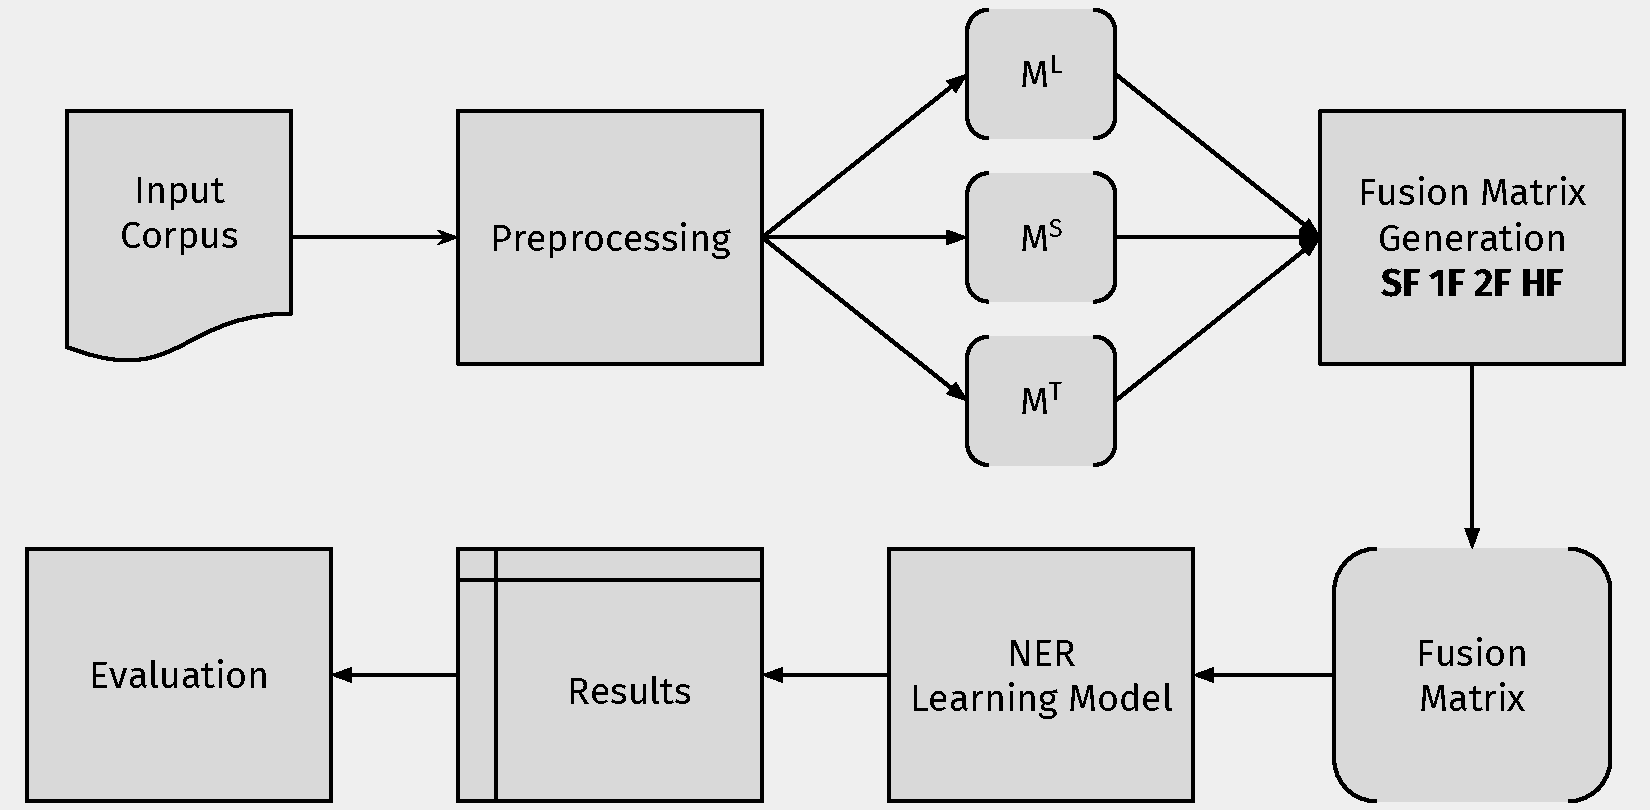
\includegraphics[width=0.85\linewidth]{image2/Chapitre4/diag_metodoNER.pdf}
%\end{frame}


\begin{frame}{Representation Spaces}
\large \textbf{Lexical Space (L)}
\vspace{1cm}
\small

\begin{tabular}{ll}
	
	\hline 
	 \textbf{Word} & \textbf{Features} \\ 
	\hline 
	Australian & word:Australian, word+1:scientist, word+2:discovers\\ 
	scientist  &  word-1:Australian, word:scientist, word+1:discovers, word+2:star\\ 
	discovers & word-2:Australian, word-1:scientist, $\dots$, word+2:telescope \\ 
	star & word-2:scientist, word-1:discovers, word:star, $\dots$, word+2:telescope \\ 
	with & word-2:discovers, word-1:star, word:with, word+1:telescope \\ 
	telescope  &  word-2:star, word-1:with, word:telescope \\ 
	\hline \
\end{tabular} 
\vspace{\textheight}
\end{frame}


\begin{frame}{Representation Spaces}
	\large \textbf{Syntactic Space (S)}
	\vspace{1cm}
	\small
	
	
	\begin{tabular}{ll}
	\hline 
	 Word & Contexts \\ 
	\hline 
	Australian & scientist/NN/amod\_inv \\ 
	scientist  &  Australian/JJ/amod, discovers/VBZ/nsubj\_inv\\ 
	discovers & scientist/NN/nsubj, star/NN/dobj, telescope/NN/nmod:with \\ 
	star & discovers/VBZ/dobj\_inv \\ 
	telescope  &  discovers/VBZ/nmod:with\_inv \\ 
	\hline \
	\end{tabular} 
	 
	\vspace{\textheight}
\end{frame}



\begin{frame}{Representation Spaces}
	\large \textbf{Standard Features Space (T)}
	\vspace{1cm}
	\begin{itemize}
		\item Each word
		\item Whether it is capitalized
		\item Prefix and suffix (of each word their surroundings)
		\item Part of Speech tag
	\end{itemize}	 
	\vspace{\textheight}
\end{frame}



\begin{frame}{Experimental Protocol}
	\begin{itemize}
		\item \large \textbf{Preprocessing}
			\begin{itemize}
				\item Normalize numbers
			\end{itemize}
		\item \textbf{Test Corpora}
			\begin{itemize}
			\item CoNLL-2003 (CONLL) \cite{SangM03}: Train: 219,554 lines. Test: 50,350 
			\item Wikiner (WNER) \cite{Nothman2009}: No Train/Test split. 3.5 million words. Evaluated in a 5-fold CV
			\item Wikigold (WGLD) \cite{Balasuriya2009}: No Train/Test split. 41,011 words. Evaluated in a 5-fold CV
			\end{itemize}
		\item \textbf{Annotation Scheme}
			\begin{itemize}
				\item \textbf{B}eginning, \textbf{I}nside, \textbf{O}utside
			\end{itemize}
		\item \textbf{Learning Algorithm}
			\begin{itemize}
				\item Structured Perceptron \cite{Collins2002}
			\end{itemize}

		\item \textbf{Evaluation Metrics}
			\begin{itemize}
				\item Precision, Recall, F-measure
			\end{itemize}
	\end{itemize}	 
	\vspace{\textheight}
\end{frame}

%\begin{frame}{Evaluation}
%\textbf{F-measure on the three datasets using single features independently with the structured perceptron}
%\vspace{1cm}
%\begin{center}
%	\begin{tabular}{@{}lccc@{}}
%	\toprule
%	$A$                           & \multicolumn{3}{c}{\textbf{Single Features}} \\ \midrule
%	                & \textbf{CONLL}    & \textbf{WNER}     & \textbf{WGLD}    \\ \cmidrule{2-4}
%	$\mstd$                        & \textbf{77.41}    & \textbf{77.50}    & \textbf{59.66}   \\
%	$\mlex$                       & 69.40    & 69.17    & 52.34   \\
%	$\msyn$                        & 32.95    & 28.47    & 25.49   \\ \bottomrule
%	\end{tabular}
%\end{center}
%\vspace{\textheight}
%\end{frame}


%\begin{frame}[t]{Evaluation}
%\textbf{F-measure on the three datasets using First Degree (1F)  fusion operators}
%\vspace{1cm}
%\begin{columns}
%\column{0.5\textwidth}
%\begin{minipage}[c][0.5\textheight][c]{\linewidth}
%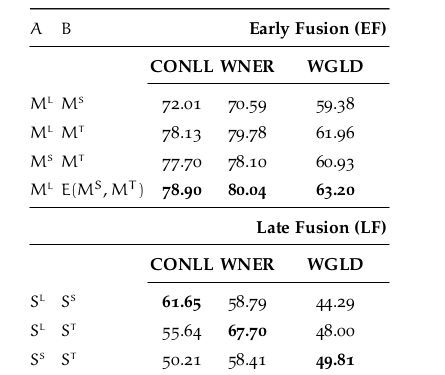
\includegraphics[width=1\linewidth]{image2/Chapitre4/1F_1.png}
%\end{minipage}
%\column{0.5\textwidth}
%\begin{minipage}[c][0.5\textheight][c]{\linewidth}
%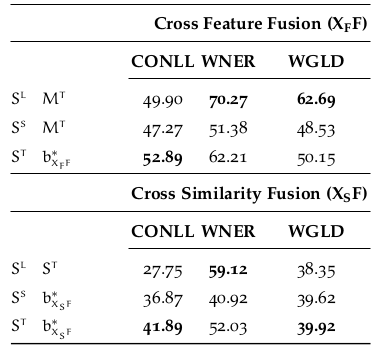
\includegraphics[width=1\linewidth]{image2/Chapitre4/1f_2.png}
%\end{minipage}
%\end{columns}
%
%\vspace{\textheight}
%\end{frame}

%\begin{frame}[t]{Evaluation}
%\textbf{F-measure on the three datasets using Second Degree (2F)  fusion operators}
%\vspace{.3cm}
%\begin{columns}
%\column{0.5\textwidth}
% \small In $X_FX_SF$, $\hat{a}$ corresponds to the best performing matrix in the set $\{ X_S(\sstd, \slex),X_S(\slex, \sstd), \allowbreak X_S(\sstd, \ssyn)\}$
%\begin{minipage}[c][0.5\textheight][c]{\linewidth}
%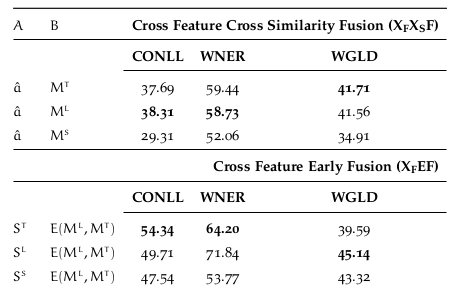
\includegraphics[width=1\linewidth]{image2/Chapitre4/2F_1.png}
%\end{minipage}
%\column{0.5\textwidth}
%In $EX_FF$, $b^*_{\scriptscriptstyle EX_FF}$  $\in$ $\{X_F(\ssyn, \mlex), \allowbreak X_F(\slex, \mlex), X_F(\slex, \mstd), \allowbreak X_F(\ssyn, \mlex), X_F(\ssyn, \mstd) \}$
%\begin{minipage}[c][0.5\textheight][c]{\linewidth}
%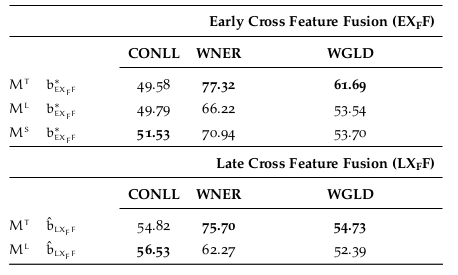
\includegraphics[width=1\linewidth]{image2/Chapitre4/2F_2.png}
%\end{minipage}
%\end{columns}
%
%\vspace{\textheight}
%\end{frame}


\begin{frame}[t]{Evaluation}

\begin{itemize}
\item Best Fusion operators on the F-measure over the three datasets.  
\item Achieved using a higher Degree fusion operator
\item Notice the comparison with the Early Fusion baseline
\item Visually show the best fusion operator, not with the formula.
\end{itemize}
\textbf{}

% \small In $EEELX_FLX_F$, $\hat{b}_{\scriptscriptstyle EEELX_FLX_F} \in  E(E(\mstd, 	 L(\mlex, X_F(\ssyn, \mlex))), \allowbreak L(\mlex, X_F(\sstd, \mlex))), E(E(\mstd, 	 L(\mstd, X_F(\ssyn, \mstd)))\allowbreak, L(\mlex, X_F(\ssyn, \mlex)))$ for CONLL, WNER and WGLD.
\begin{center}
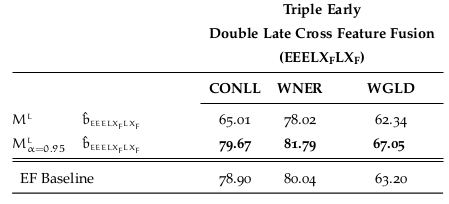
\includegraphics[width=0.6\linewidth]{image2/Chapitre4/hf_trim.png}
\end{center}


\vspace{\textheight}
\end{frame}

\begin{frame}{Analyzing the Best Fusion Operator}
Decompose best fusion in four models:
\begin{equation*}
\overbrace{\underbrace{\overbrace{E_{\alpha=0.95}(\underbrace{\mlex}_{\circled{1}},\mstd}^{\circled{2}},L(\mstd, X_F(\ssyn, \mstd))}_{\circled{3}}, L(\mlex, X_F(\ssyn, \mlex))}^{\circled{4}})
\end{equation*}
\begin{enumerate}
\item[\circled{1}] $\mlex$ \label{eq:f1} used to train model $M_1$.
\item[\circled{2}] $E(\alpha_1\mlex, \alpha_2\mstd)$ \label{eq:f2} used to train model $M_2$, with $\alpha_1=0.95,\alpha_2=0.05$
\item[\circled{3}] $E_\alpha(\alpha_1\mlex, \alpha_2\mstd, \alpha_3L(\mstd, X_F(\ssyn, \mstd)))$ used to train model $M_3$, with $\alpha_1=0.95,\alpha_2=\alpha_3=0.05$
\item[\circled{4}] $E_\alpha(\alpha_1\mlex, \alpha_2\mstd, \alpha_3L(\mstd, X_F(\ssyn, \mstd)), \alpha_4L(\mlex, X_F(\ssyn, \mlex)))$ used to train model $M_4$, with $\alpha_1=0.95,\alpha_2=\alpha_3=\alpha_4=0.05$
\end{enumerate}
\end{frame}


\begin{frame}{Analyzing the Best Fusion Operator}
\large \textbf{We focus on the word \textit{Kory}, and its performance from model $M_1$ to $M_2$}
\begin{center}
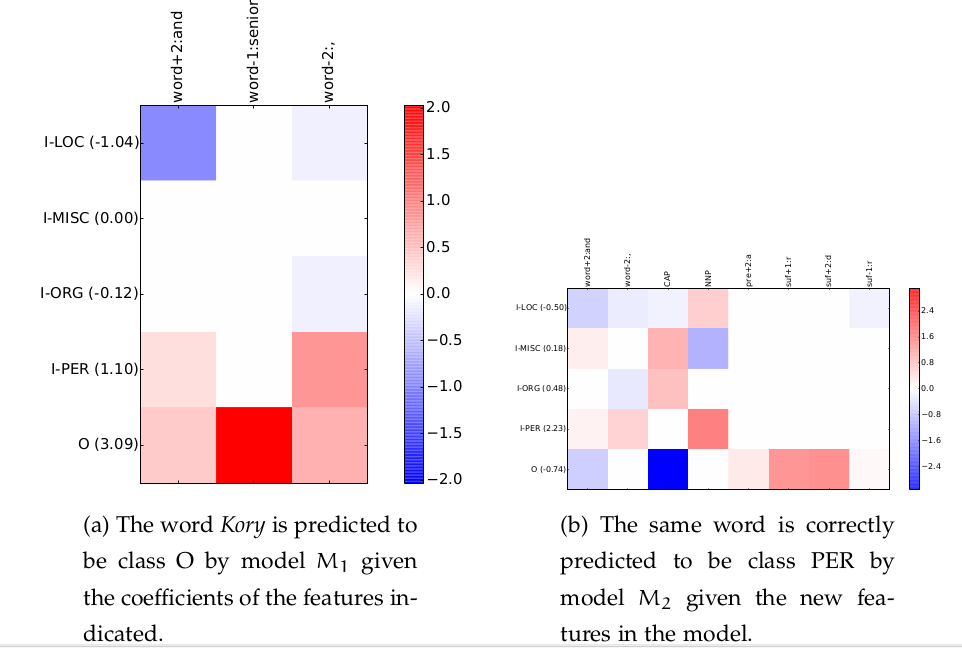
\includegraphics[width=0.6\linewidth]{image2/Chapitre4/fanal1.png}
\end{center}
\end{frame}


\begin{frame}{Analyzing the Best Fusion Operator}
\large \textbf{We focus on the word \textit{Green}, and its performance from model $M_3$ to $M_4$}
\begin{center}
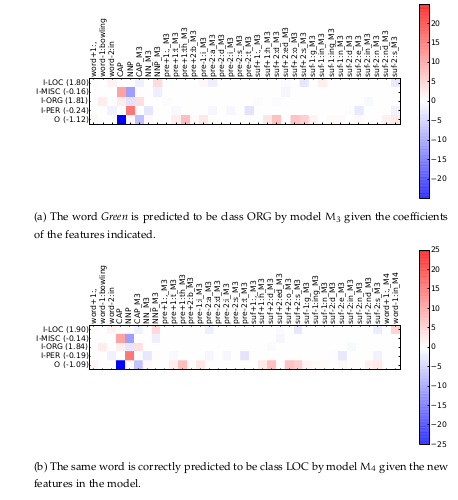
\includegraphics[width=0.6\linewidth]{image2/Chapitre4/fanalm3_m4.png}
\end{center}
\end{frame}

\section[Applications to NLP]{Solving Word Sense Induction and Disambiguation}

\subsection{Word Sense Induction and Disambiguation}
\begin{frame}{Introduction}
\begin{center}
\begin{itemize}
\item Introduction to WSI/WSD
\end{itemize}
%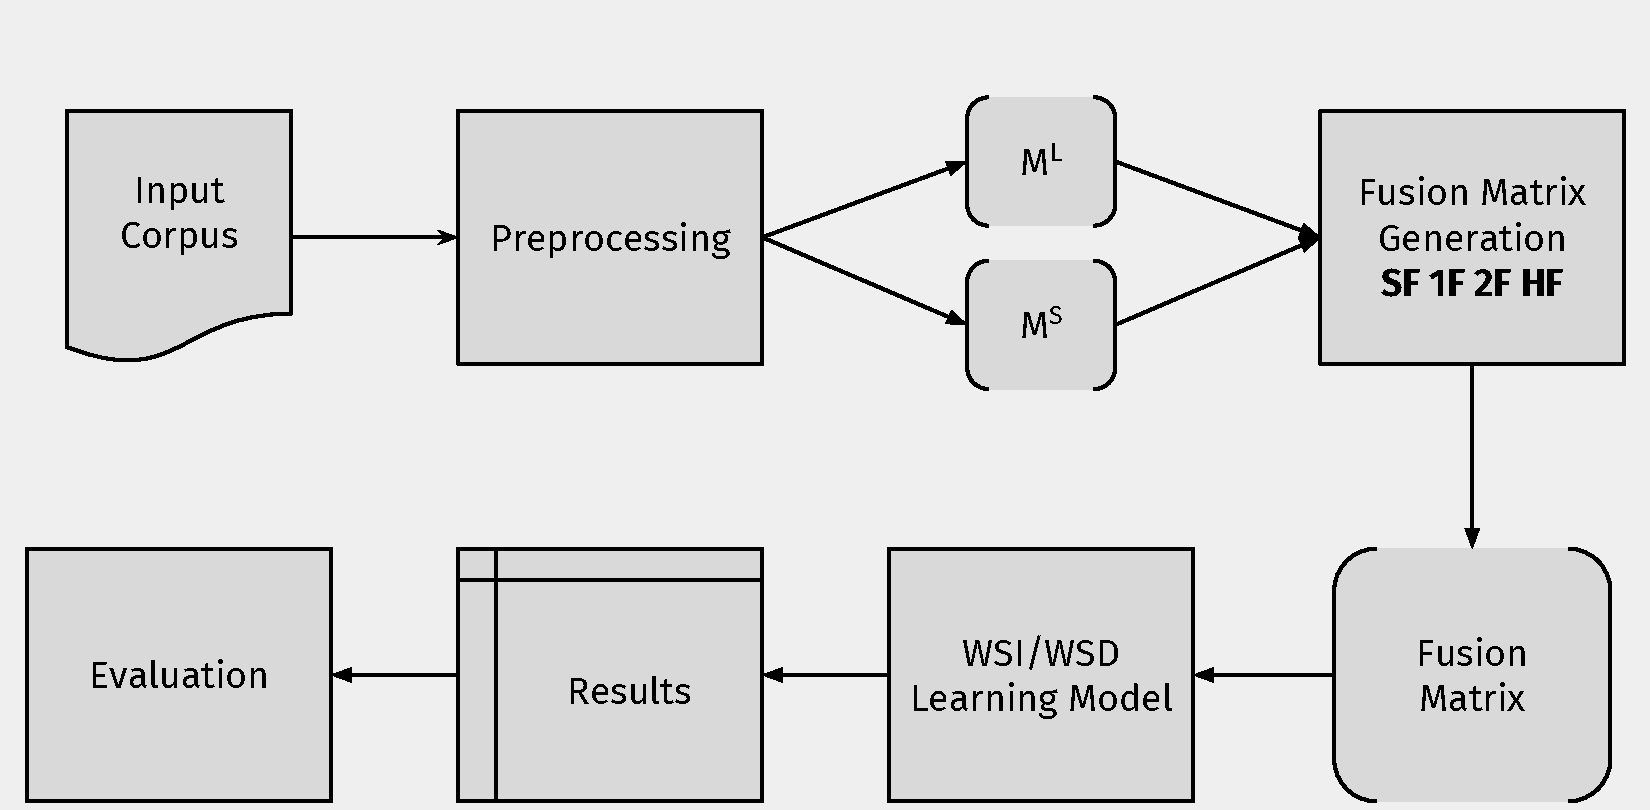
\includegraphics[width=0.9\linewidth]{image2/Chapitre4/diag_metodoWSD.pdf}
\end{center}
\end{frame}


\begin{frame}{Experimental Protocol}
	\begin{itemize}
		\item \large \textbf{Preprocessing}
			\begin{itemize}
				\item Normalize numbers
			\end{itemize}
		\item \textbf{Test Corpora}
			\begin{itemize}
			\item Semeval 2007 \cite{SangM03}: Train: 219,554 lines. Test: 50,350 
			\end{itemize}
		\item \textbf{Clustering Algorithm}
			\begin{itemize}
				\item Spectral Clustering
			\end{itemize}

		\item \textbf{Evaluation Metrics}
			\begin{itemize}
				\item Supervised: F-score
				\item Unsupervised: Recall
				\item Proposed: H-score
			\end{itemize}
	\end{itemize}	 
	\vspace{\textheight}
\end{frame}

\begin{frame}{WSI/WSD: Evaluation}
\begin{itemize}
\item Results for WSI/WSD with spectral clustering
\end{itemize}
\end{frame}



\begin{frame}{Finding Senses in the Network}

	\large  \textbf{How to exploit a linguistic network to solve word sense induction and disambiguation?}
	\vspace{.5cm}
	\normalsize
	\begin{itemize}
		\item \textbf{Similar approaches}
			\begin{itemize}
				\item Hyperlex \cite{2004.Veronis}
				\item University of York (UoY) \cite{2007.Klapaftis.UOY}
			\end{itemize}
		\item \textbf{Limitations of existing approaches}
		\begin{itemize}
			\item Single typed networks
			\item Large number of parameters
		\end{itemize}
		\item \textbf{Features}
		\begin{itemize}
				\item Be able to exploit different types of linguistic information (lexical or syntactic co-occurrence)
				\item Keep  the number of parameters low and allow for their automatic adjusting according to the network's nature
%				\item Use a robust and interpretable similarity measure
		
		\end{itemize}
\end{itemize}
\vspace{\textheight}	
\end{frame}
\begin{frame}{Proposed Method}
  \centering
  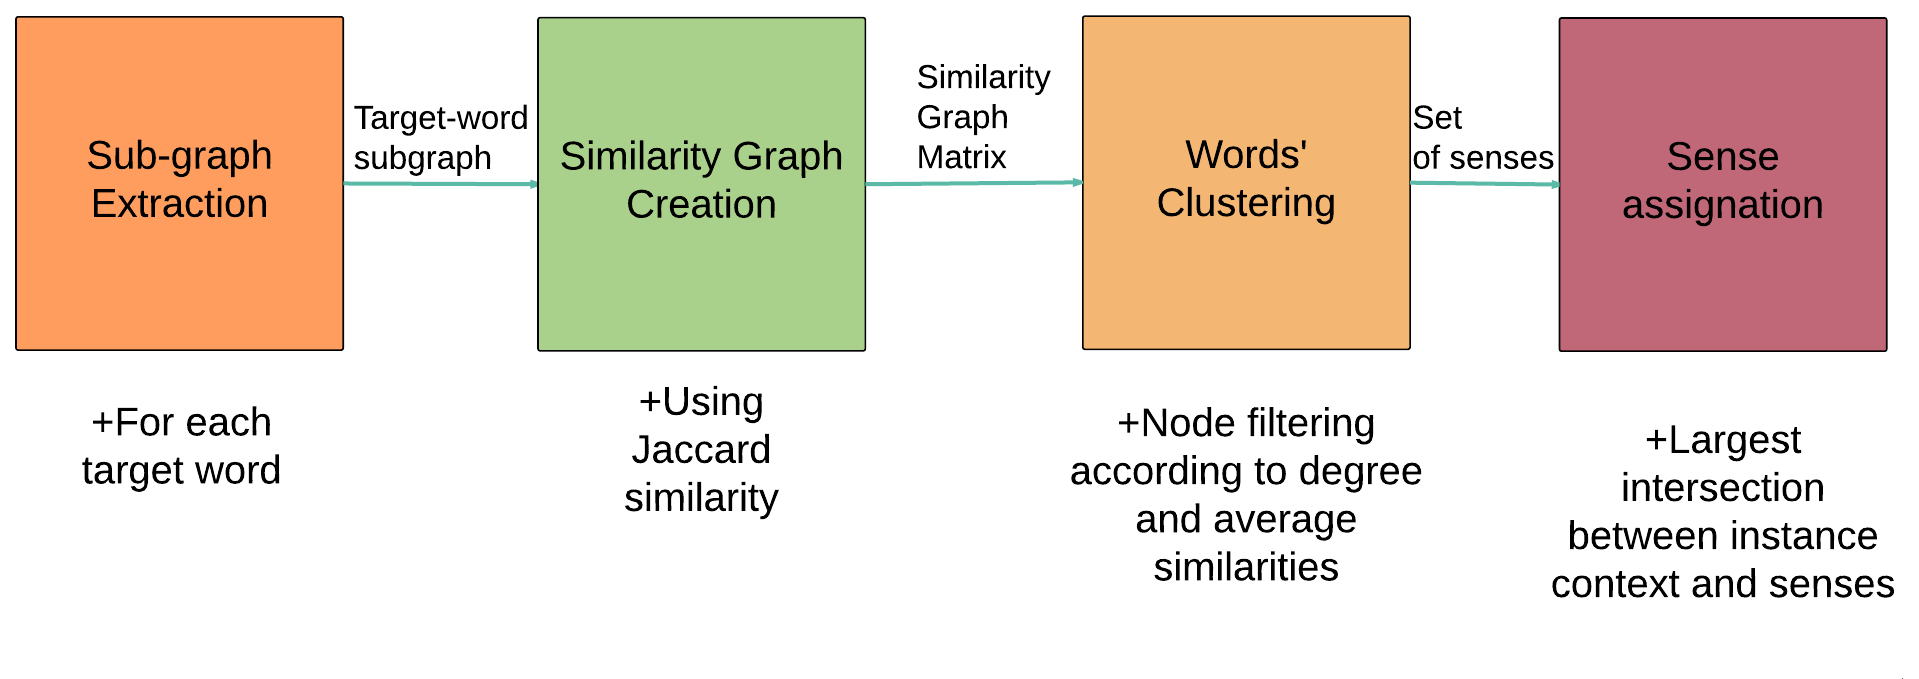
\includegraphics[width=1\linewidth]{img/wsd_wsi.png}

\end{frame}









\begin{frame}{Semeval Results}
\begin{itemize}
\item Semeval 2007 results table
\end{itemize}
\end{frame}






\begin{frame}{WSI/WSD: Evaluation}
\begin{itemize}
\item Verbs and nouns behaviors
\item Insight into senses found by the algorithm
\end{itemize}
\end{frame}
%
%
%
%\item\textbf{ How can we improve the model?}
%\begin{itemize}
%\item Leverage large sources of text data to enrich current approach
%\item Combine the information stored in the HLM
%\item Improve the WSD stage
%\item Select other more pertinent similarity measures
%
%\end{itemize}
%





%
%


%\section{Ongoing Work}
%
%
%
%\begin{frame}{Combining linguistic features: Information Fusion}
%%			\item By projecting robust information from the syntactic dependencies hypergraph incidence matrix towards the lexical co-occurrence incidence matrix, via the dot product, we can propagate the information contained in the first matrix into the second and thus find more relevant semantic relations between words.
%%			
%%			\begin{figure}
%%			\centering
%%			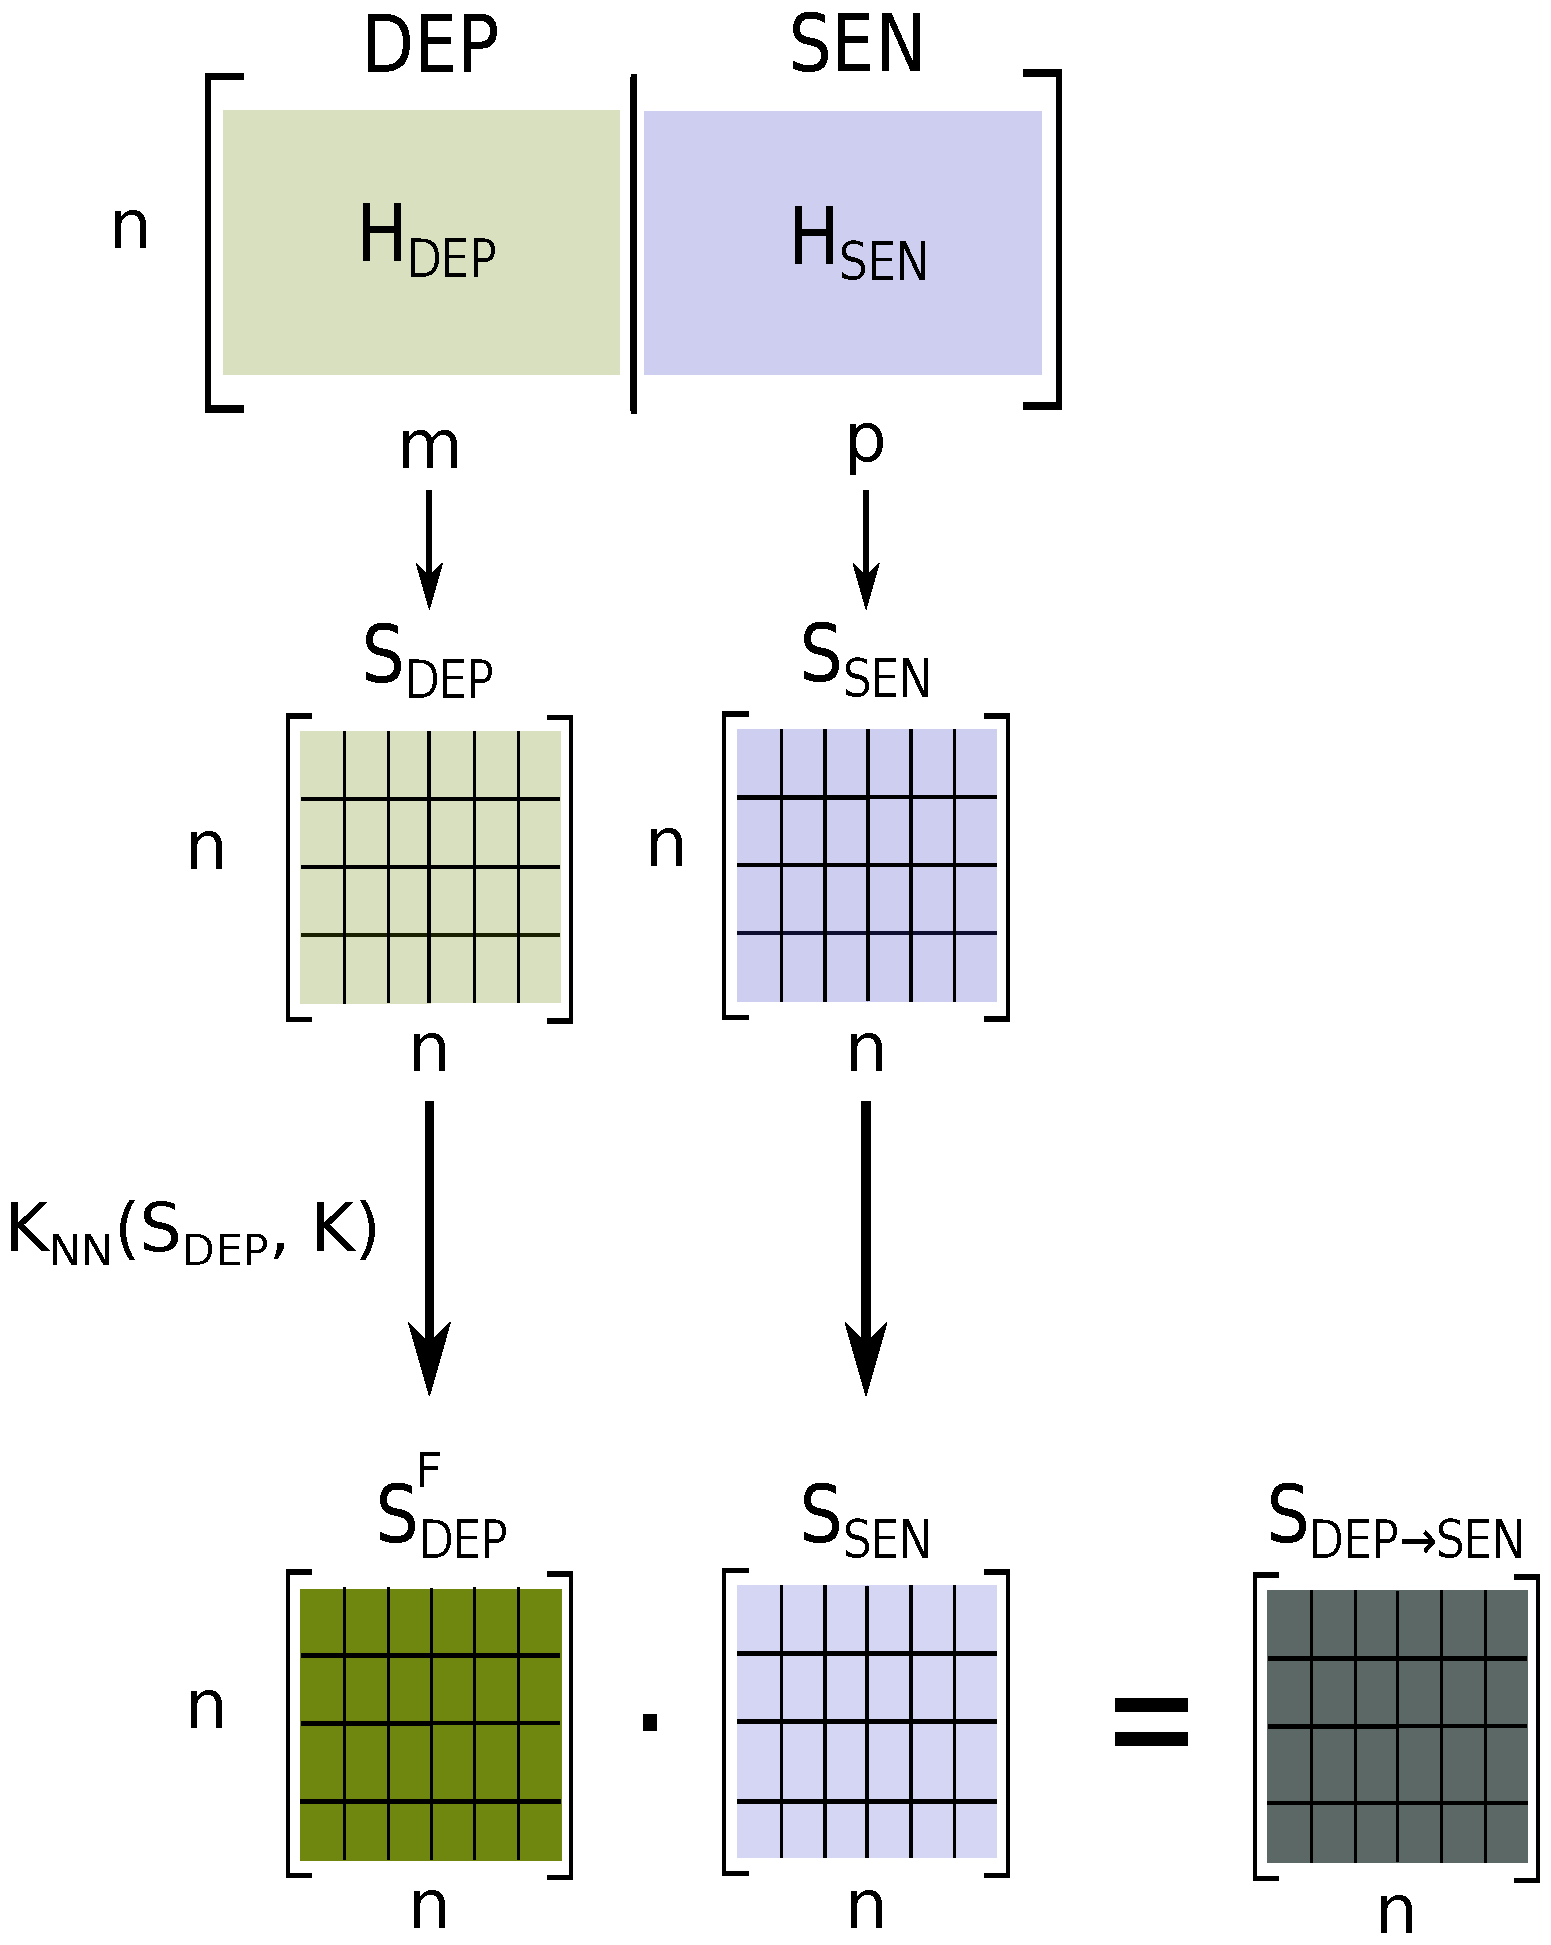
\includegraphics[width=0.4\linewidth]{img/cross}
%%			\end{figure}
%
%
%	\begin{columns}
%	\column{.5\textwidth}
%	\begin{minipage}[c][0.4\textheight][c]{\linewidth}
%	  \centering
%	  \begin{itemize}
%		  \item \textbf{Inspired on the image/text fusion literature \cite{Snoek2005,ah2015unsupervised}:}
%		  \begin{itemize}
%			  \item Early fusion
%			  \item Late fusion
%			  \item \textbf{Cross fusion}
%		  
%		  \end{itemize}
%	  
%	  \end{itemize}
%	\end{minipage}
%	\column{.5\textwidth}
%	\begin{minipage}[c][0.4\textheight][c]{\linewidth}
%		\centering
%		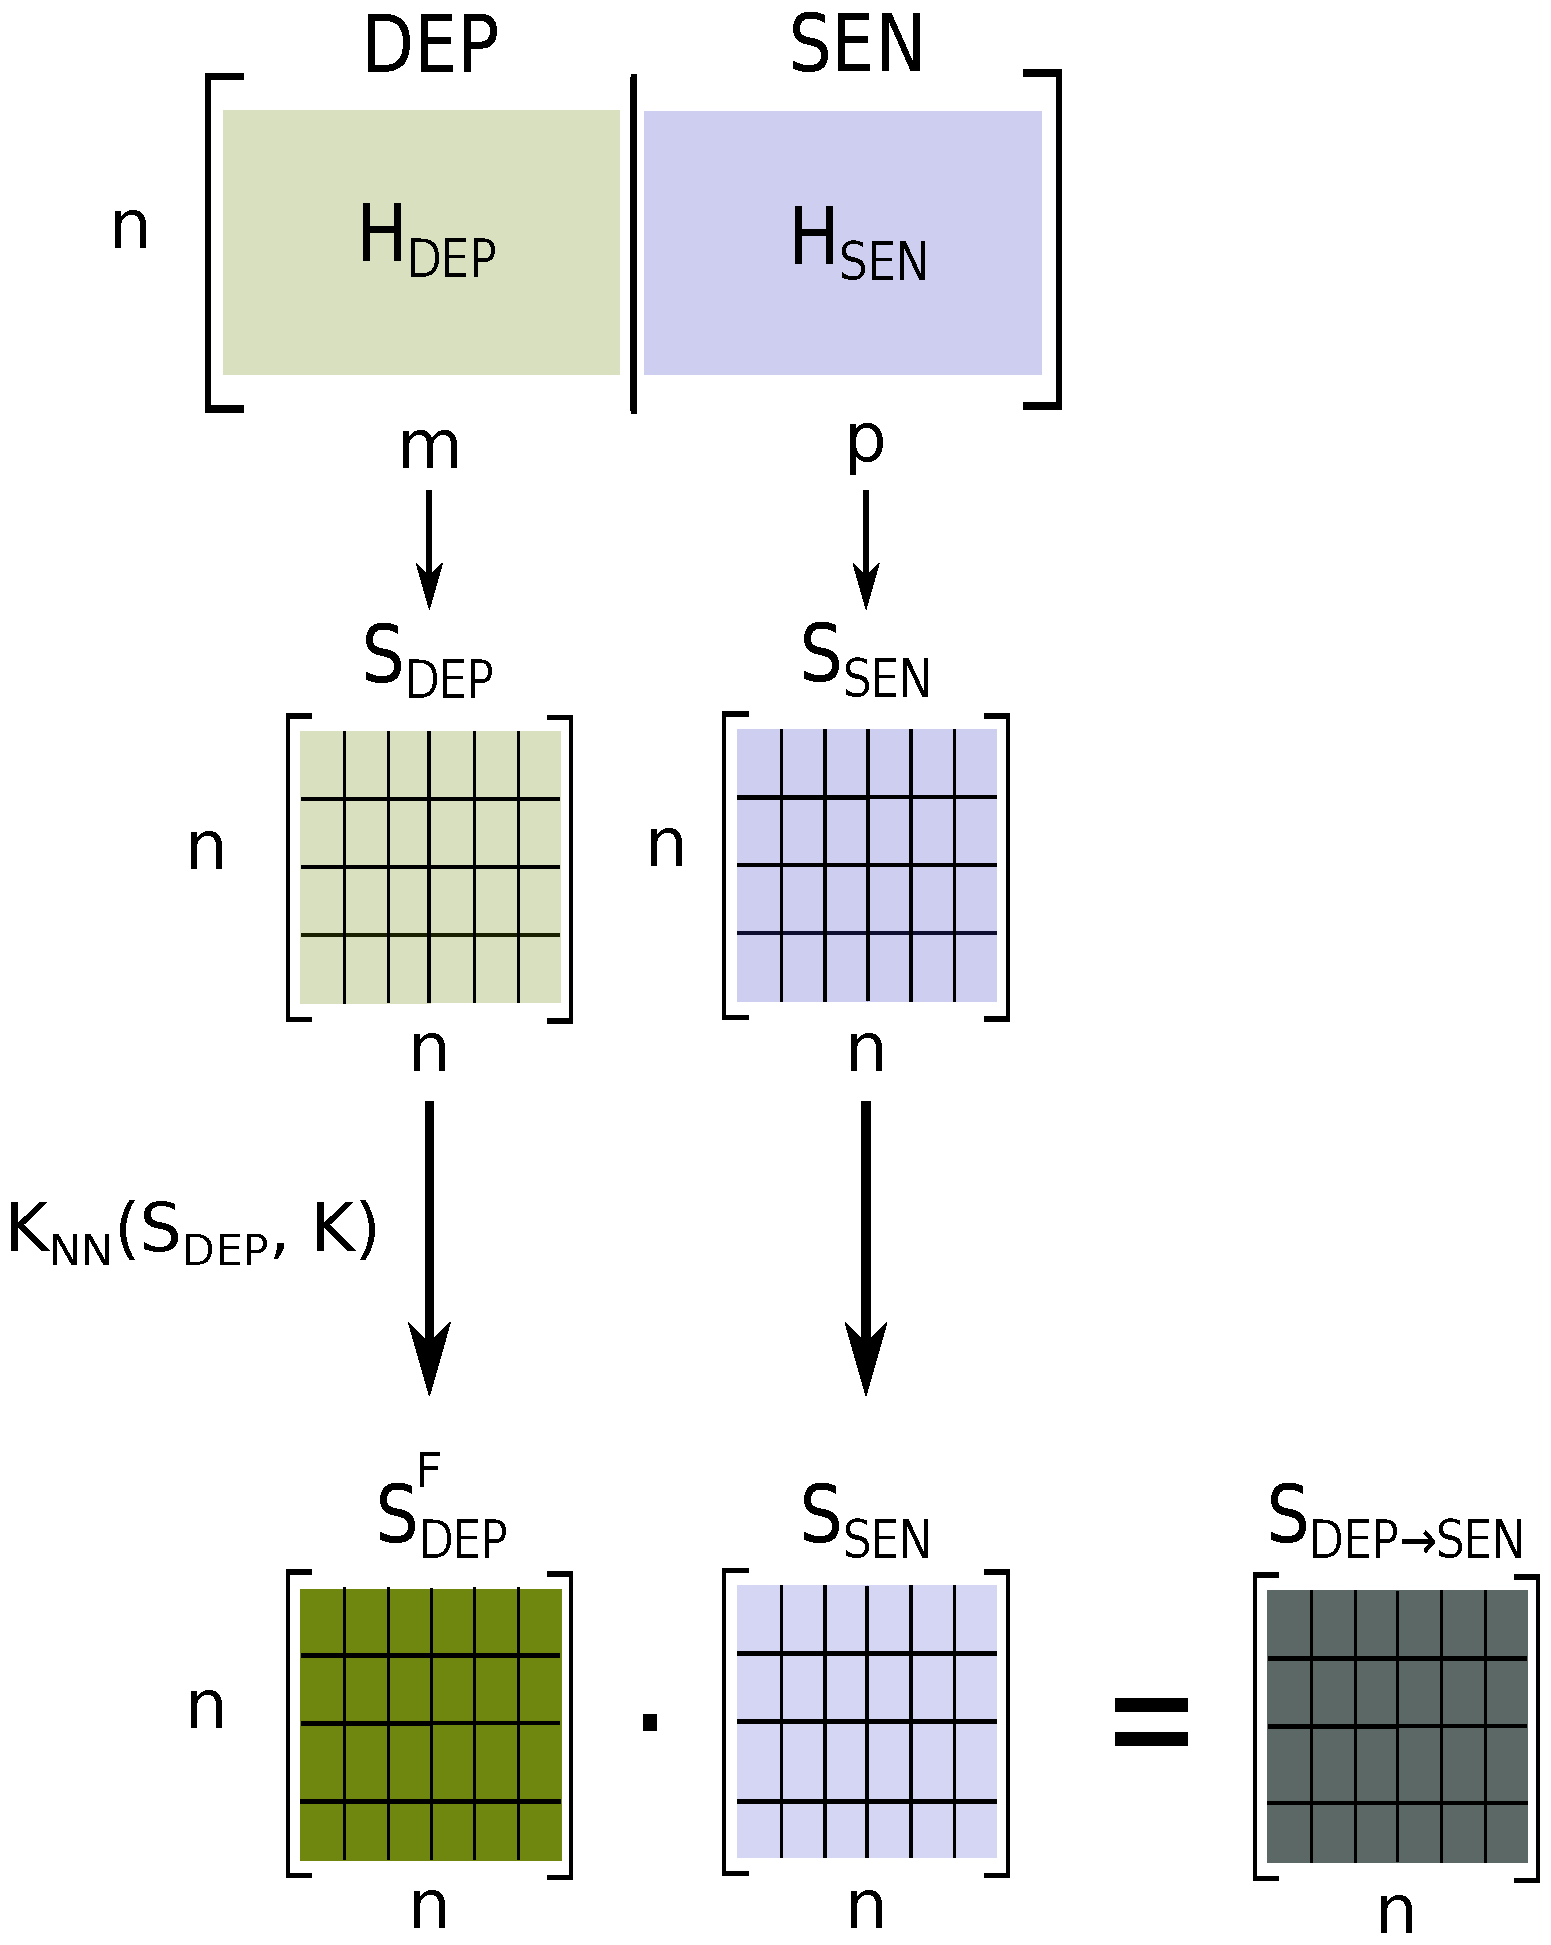
\includegraphics[width=1\linewidth]{img/cross}
%	\end{minipage}
%	\end{columns}
%
%			
%\end{frame}
%



\section{Conclusions}

\begin{frame}{Insights From our Contributions}
%\begin{itemize}
%	\item \textbf{Hypergraph Linguistic Model}
%		\begin{itemize}
%			\item Takes into account different types of linguistic information
%			\item Link multiple words together
%		\end{itemize}
%	\item \textbf{WSD and WSI method based on a HLM}	
%		\begin{itemize}
%			\item Use syntactical or lexical co-occurrences
%			\item Take into account network nature and reduce number of parameters
%		\end{itemize}
%	\item \textbf{Building a syntactically parsed Wikipedia dump}	
%			\begin{itemize}
%				\item Contains constituents information missing from most Wikipedia parses
%				\item Fits with our proposed HLM model
%			\end{itemize}
%			
%		
%\end{itemize}


\end{frame}





\begin{frame}{Future Work}
%
%\begin{itemize}
%\item \textbf{WSD and WSI}
%\begin{itemize}
%	\item Further explore the combination of linguistic features 
%	\item Look into applying a better WSD technique
%	\item Interpret the results from a qualitative point of view 
%\end{itemize}
%
%\item \textbf{Information Extraction}
%\begin{itemize}
%	\item Apply the semantic knowledge obtained until now to solve Named Entity Recognition
%	\item Enrich our techniques with open access textual information
%\end{itemize}
%\end{itemize}
%
%\end{frame}
%
%\begin{frame}{The End}
%\large Thank you for your attention

\end{frame}
	
\begin{frame}[allowframebreaks]{References}

\printbibliography
%\bibliographystyle{alpha}

\end{frame}	
	
\end{document}
